
\documentclass[english,11pt]{article}

\usepackage[margin=1in]{geometry} 
\usepackage{amsmath,amsthm,amssymb}
\usepackage{graphicx}
\usepackage{float}
\usepackage{amsmath}
\usepackage{breqn}
\usepackage{amssymb}
\usepackage{mhchem}
\usepackage{fancyhdr}
\usepackage{mathrsfs}
\usepackage{euscript, eufrak}
\usepackage{pdfpages}
\pagestyle{fancy}
\usepackage{babel, blindtext}
\usepackage{subcaption}
\usepackage{caption}
\lhead{Problem Set 1}
\rhead{Saundra Albers}
\newcommand{\N}{\mathbb{N}}
\newcommand{\Z}{\mathbb{Z}}
%\usepackage{subfig, subfloat}
%\@ifundefined{showcaptionsetup}{}{ \PassOptionsToPackage{caption=false}{subfig}}
%\usepackage{subfig, subfloat}
 
\begin{document}
 

%\renewcommand{\qedsymbol}{\filledbox}
 
\title{Problem Set 2}
\author{Saundra Albers\\ 
Astronomy 250 - Stellar Populations} 
 
\maketitle
 

\section*{Problem 1}
\textit{There is a minor mistake on the Initial Mass Function page of Wikipedia. What is it?}\\
%On the Wikipedia page for the IMF, it states under Salpeter 1955 that 'His work favored an exponent of $\alpha$ = 2.35.' However, the Salpeter 1955 paper actually reports an $\alpha$ of 1.35.
%\begin{equation}
%\xi (\mathfrak{M}) \approx 0.03 \Bigg( \frac{\mathfrak{M}}{\mathfrak{M}_{\odot}} \Bigg)^{-1.35}
%\end{equation}
In the article when they discuss the Miller-Scalo 1979 paper, it reads ' Glenn E. Miller and John M. Scalo suggested that the IMF "flattened" (approached $\alpha = 0$) below one solar mass.'
However because $\alpha$ is the exponent on $\frac{dn}{dm}$ and $\Gamma$ is the exponent on $\frac{dn}{d log(m)}$ by convention, it is $\Gamma$ that is 0, where $\alpha$ = 1.

\section*{Problem 2}
\textit{Consider a single power-law IMF of the form:}
\begin{equation}
P(M|\theta) = c M^{-\alpha}
\end{equation}
where
\begin{equation}
c = \frac{1}{\int_{M_{min}}^{M_{max}}M^{-\alpha}dM}
\end{equation}
and $\theta = (M_{min}, M_{max}, \alpha)$.
\textit{For simplicity, assume perfect knowledge of the masses and that observational effects are negligible.}\\
The code and the totality of the plots for this problem can be found in the file \textbf{ps2\_problem2.ipynb}.
\subsection*{(a)}
\textit{Write code that generates a list of N stellar masses between a given $M_{min}$ and $M_{max}$ from a power-law distribution with an index of $\alpha$.}\\
For this part of the problem, I used  a numpy function called np.random.power to generate a list of masses sampled from a power-law with slope $\alpha$. I then scaled it to the correct range of interest, between the minimum and maximum stellar masses. Below is a histogram of a sample of 10,000 masses.

\begin{figure}[H]
\centering
\caption{Histogram of Sampled Masses from a Power Law with Slope $\alpha$ = 1.35}
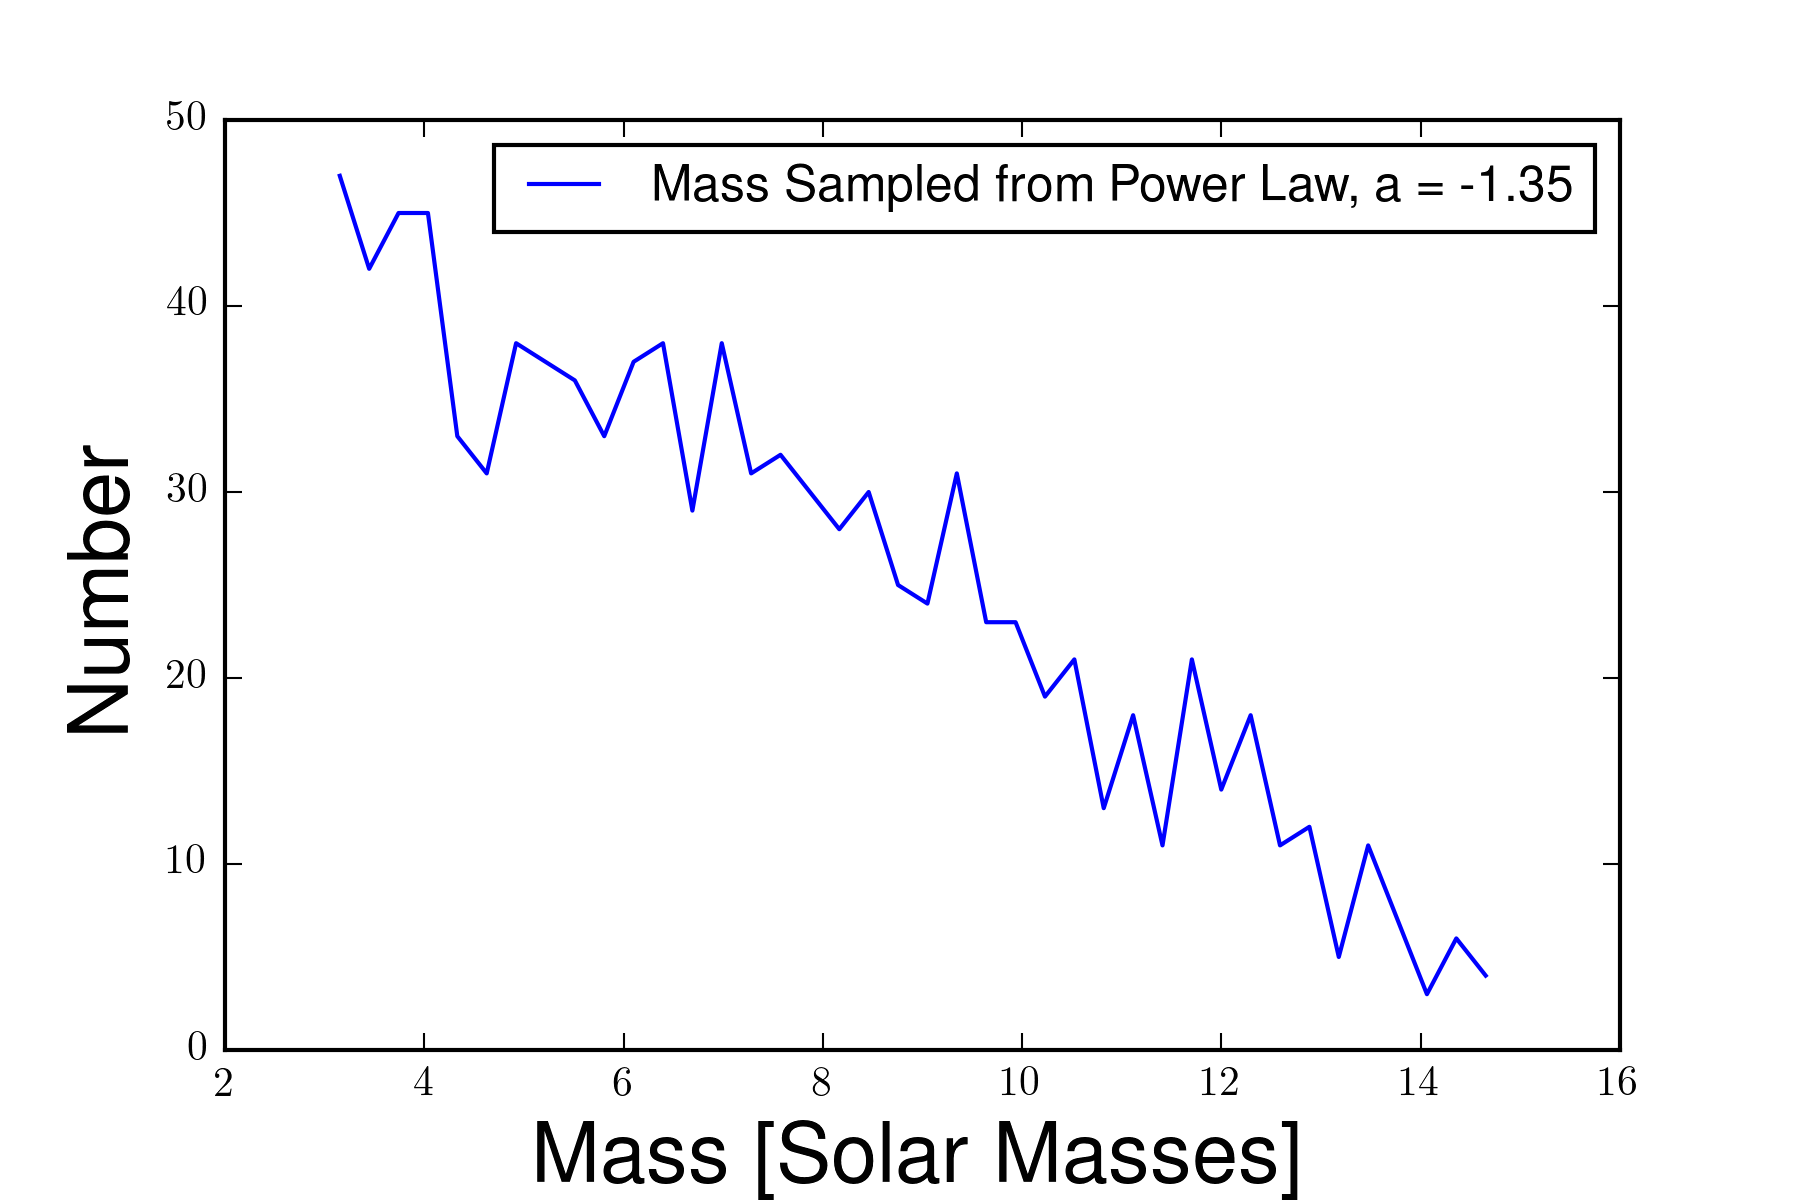
\includegraphics[scale = 0.6]{mass_histogram_prob2.png}
\end{figure}

\subsection*{(b)}
\textit{Write code that will perform inference on the set of fake data you generated in part (a) using emcee.}\\
For part b, I wrote code that performed inference on the mass data to infer a maximum mass and slope for the power law. In order to find the best fit for $\alpha$ and $M_{max}$ for the data, I fit a histogram to the sampled data and used that to compare with trial values for $\alpha$ and $M_{max}$ in the likelihood function.  I fit the data in log space to simplify the problem to a linear fit. I also assumed a flat, top hat prior where $\alpha$  is a positive value between 0 and 5.0 and $M_{max}$ must be greater that $M_{min}$ to avoid getting a negative integral in the constant.

\subsection*{(c)}
\textit{Generate a fake dataset assuming $M_{min} = 3 M_{\odot}$ and $M_{max} = 15 M_{\odot}$, N = 1000 and $\alpha$ = 1.35. In your inference code, let $\alpha$ and $M_{max}$ be free parameters (but fix $M_{min} = 3 M_{\odot}$). Given this fake dataset, to what precision can you constrain $\alpha$ and $M_{max}$? }\\
For this part of the problem I used the code developed in part (a) and (b) to find constraints on  $\alpha$ and $M_{max}$. While emcee was able to constrain the slope very well, it was unable to constrain the maximum mass. I'm unsure why this problem arose. Below are two plots that show the parameter $\alpha$ and $M_{max}$ vs. Step Number.

\begin{figure}[H]
\caption{These figures are from a 1000 mass point data set.}
\centering
\begin{subfigure}{.4\textwidth}
  \centering
  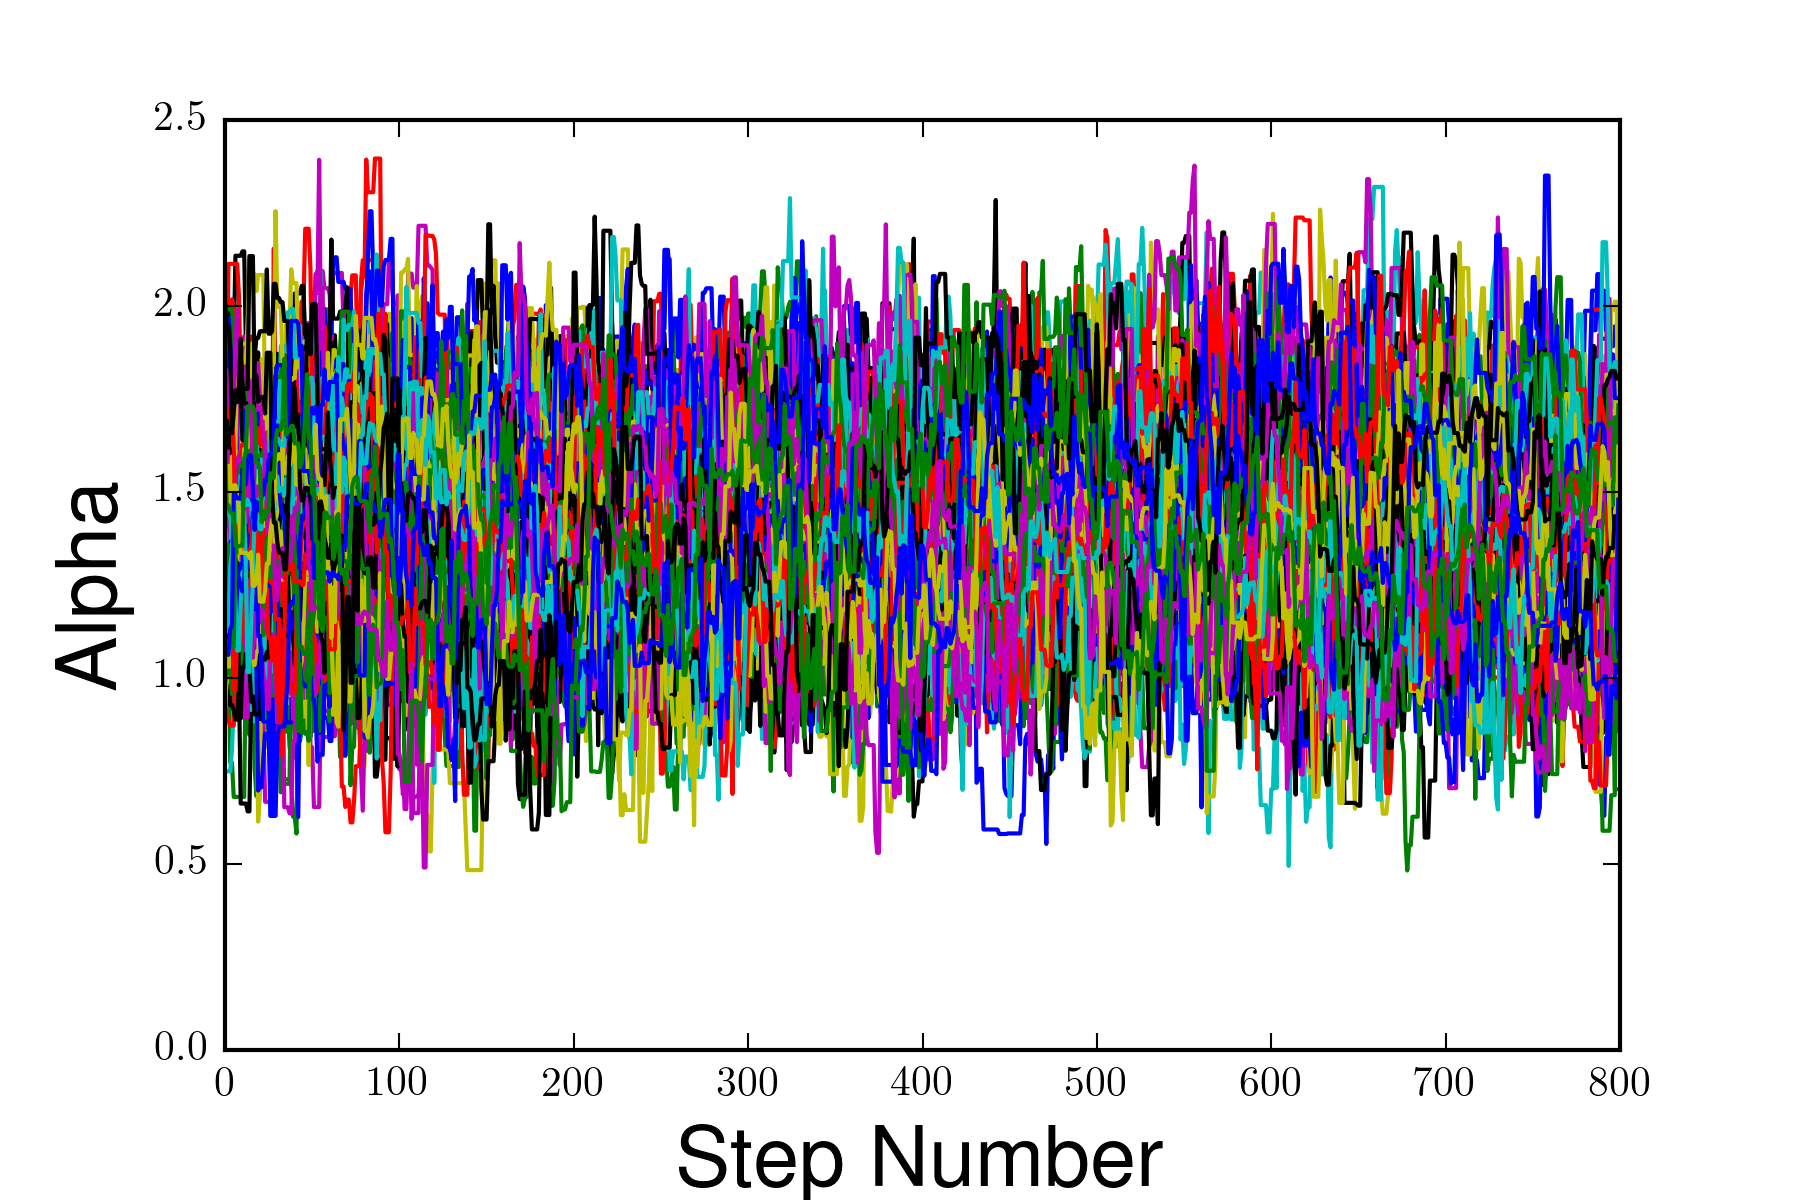
\includegraphics[width=\linewidth]{alpha_step_emcee_prob2.png}
  \caption{$\alpha$ vs. Step Number}
  \label{fig:sub1x}
\end{subfigure}%
\begin{subfigure}{0.4\textwidth}
  \centering
  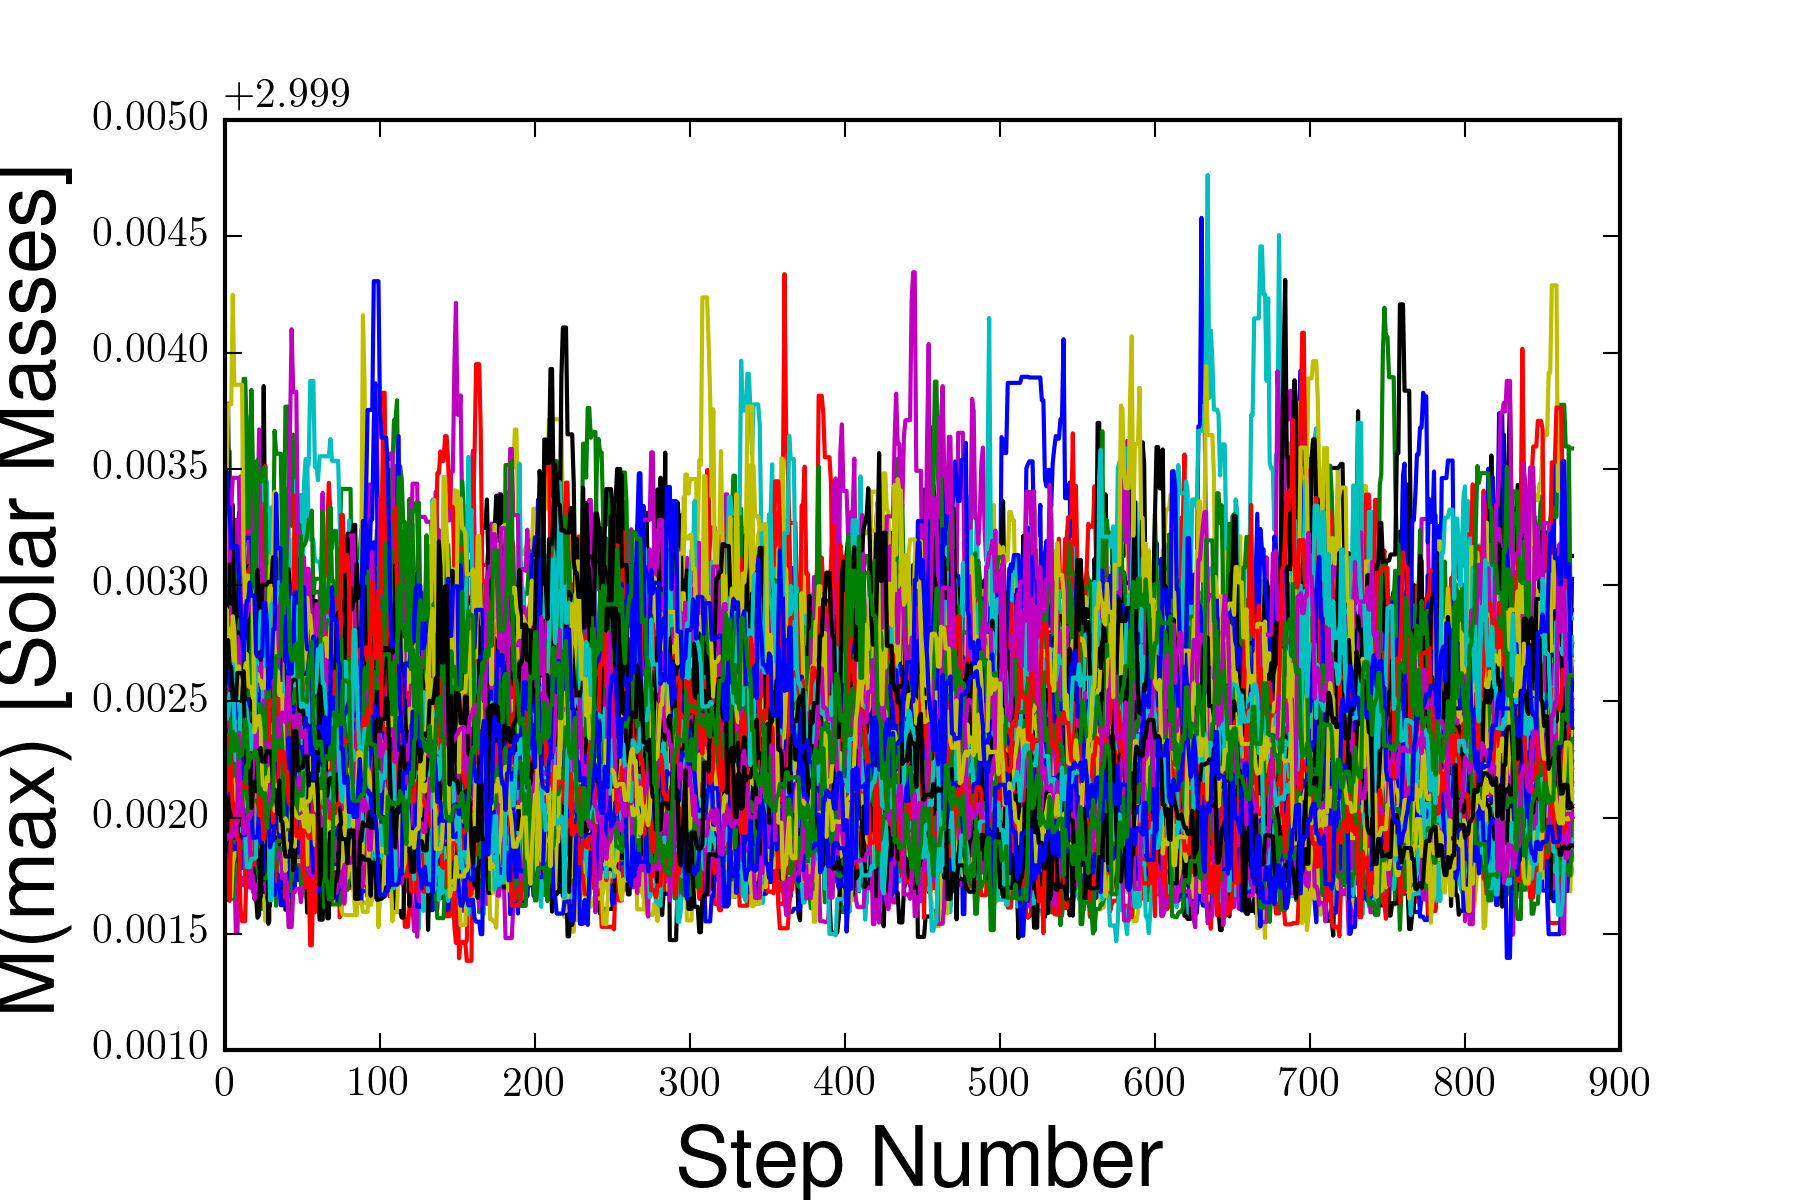
\includegraphics[width=\linewidth]{m_max_step_emcee_prob2.png}
  \caption{$M_{max}$ vs. Step Number}
  \label{fig:sub2x}
\end{subfigure}
\label{fig:testx}
\end{figure}
While it is clear that the code is converging on the correct value of the slope, the walkers seem to have trouble stepping toward a higher mass value for $M_{max}.$ This is also evidenced by the corner contour plot below. The distribution for $\alpha$ is centered at the right value, while  the value for $M_{max}$ sharply peaks at the minimum mass.

\begin{figure}[H]
\centering
\caption{Contour plot of  $\alpha$ and $M_{max}$ }
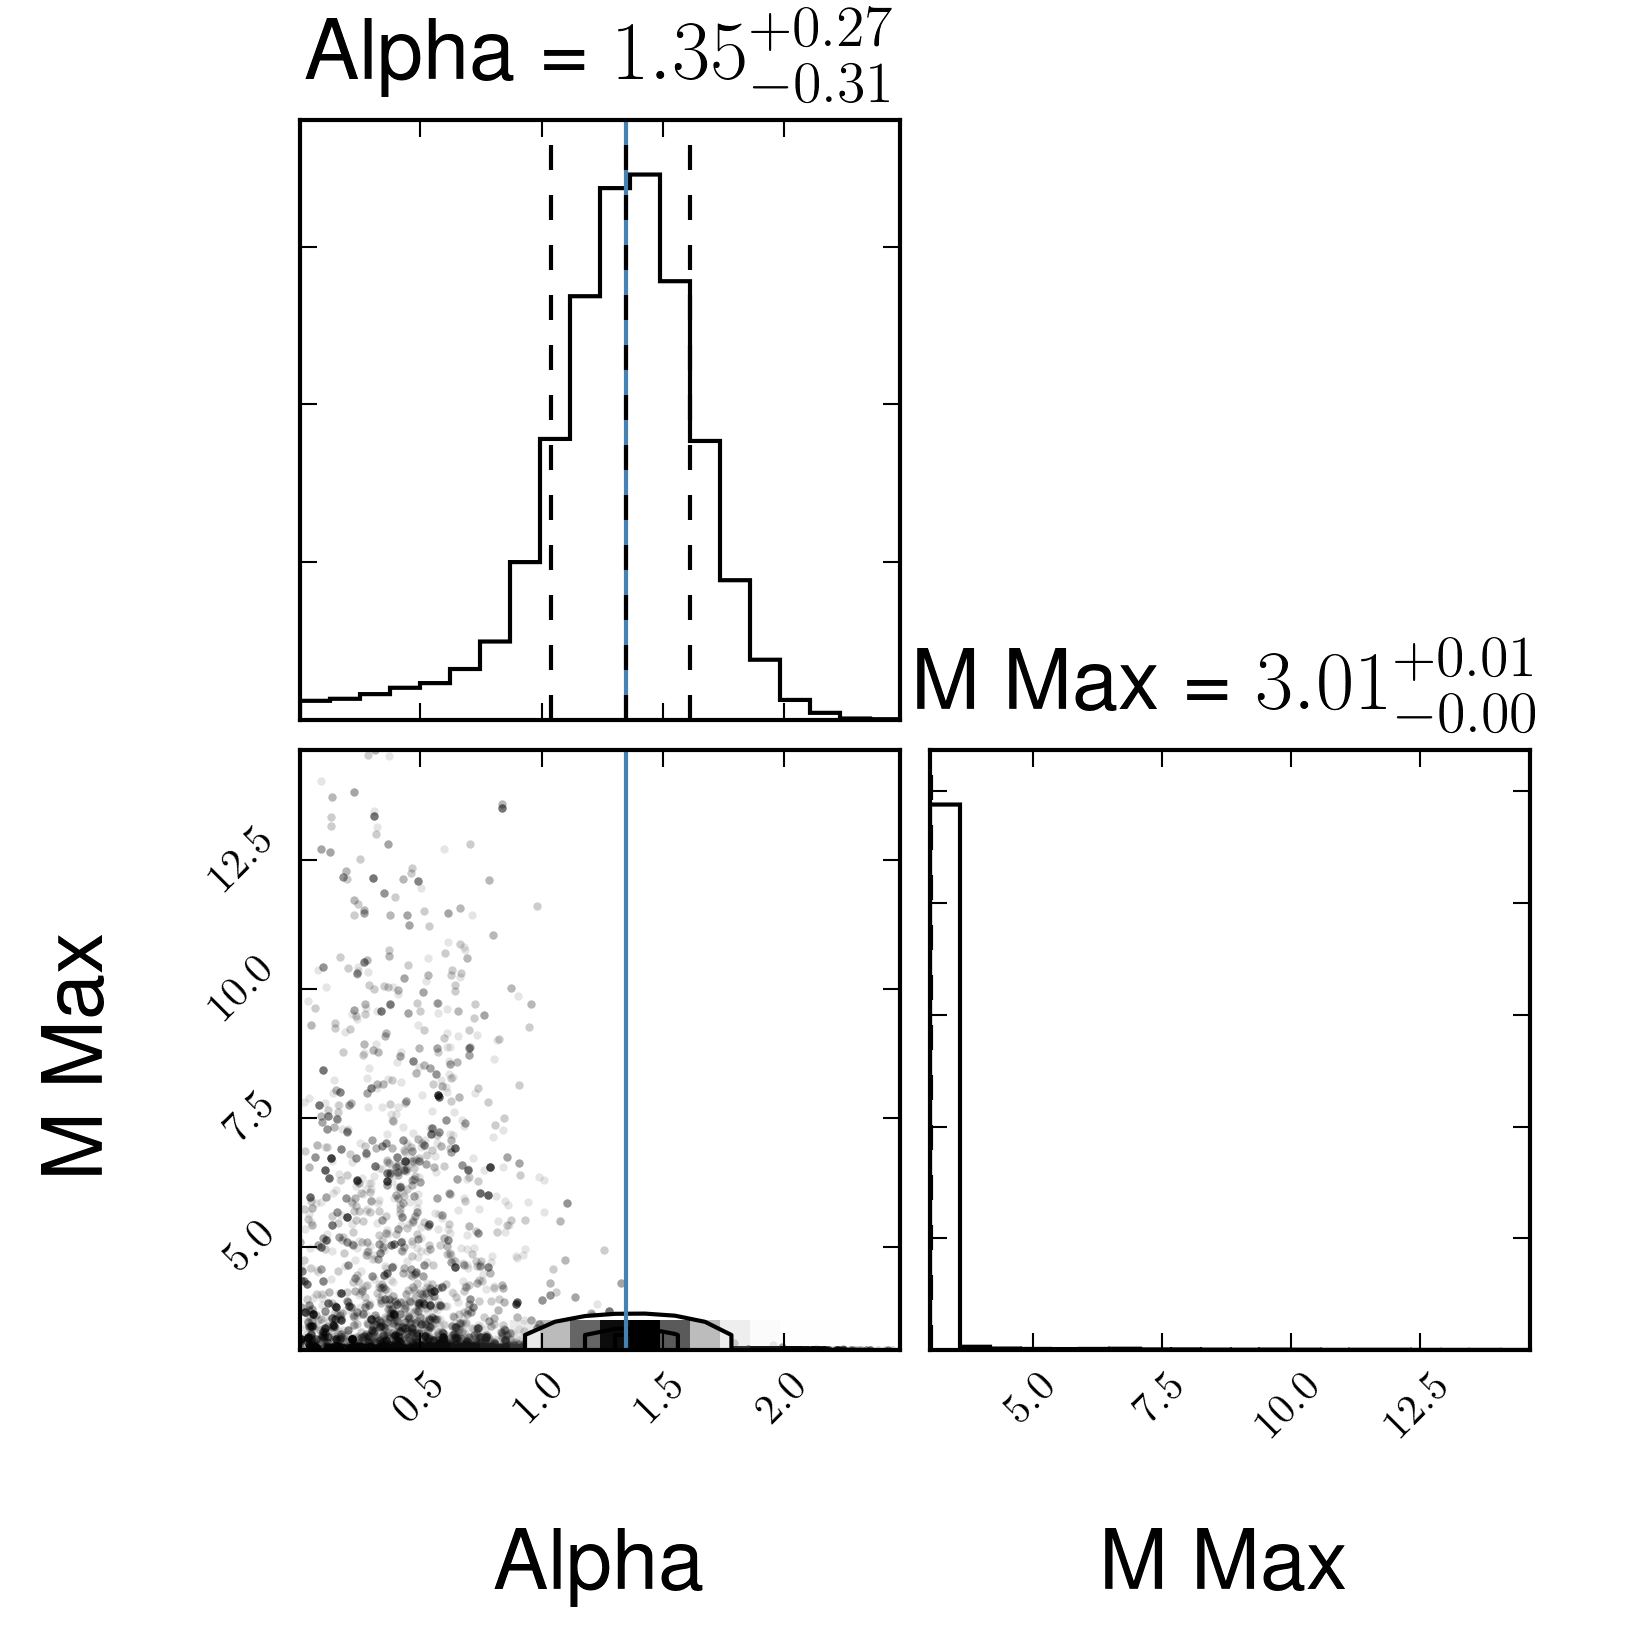
\includegraphics[scale = 0.6]{corner_plot_emcee_prob2_1000_data.png}
\end{figure}

\subsection*{(d)}
\textit{Show how the precision to which $\alpha$ and $M_{max}$ can be recovered depends on N, from N $\approx$ 10 to N $\approx$ 10,000. Summarize your results in plots.}\\
Below are histograms and contour plots from data runs of 10, 100, 1,000 and 10,000. As evidenced by the spread of the contours, the small data set runs are very inaccurate.

%\begin{figure}[H]
%\centering
%\caption{Contour plot of  $\alpha$ and $M_{max}$ }
%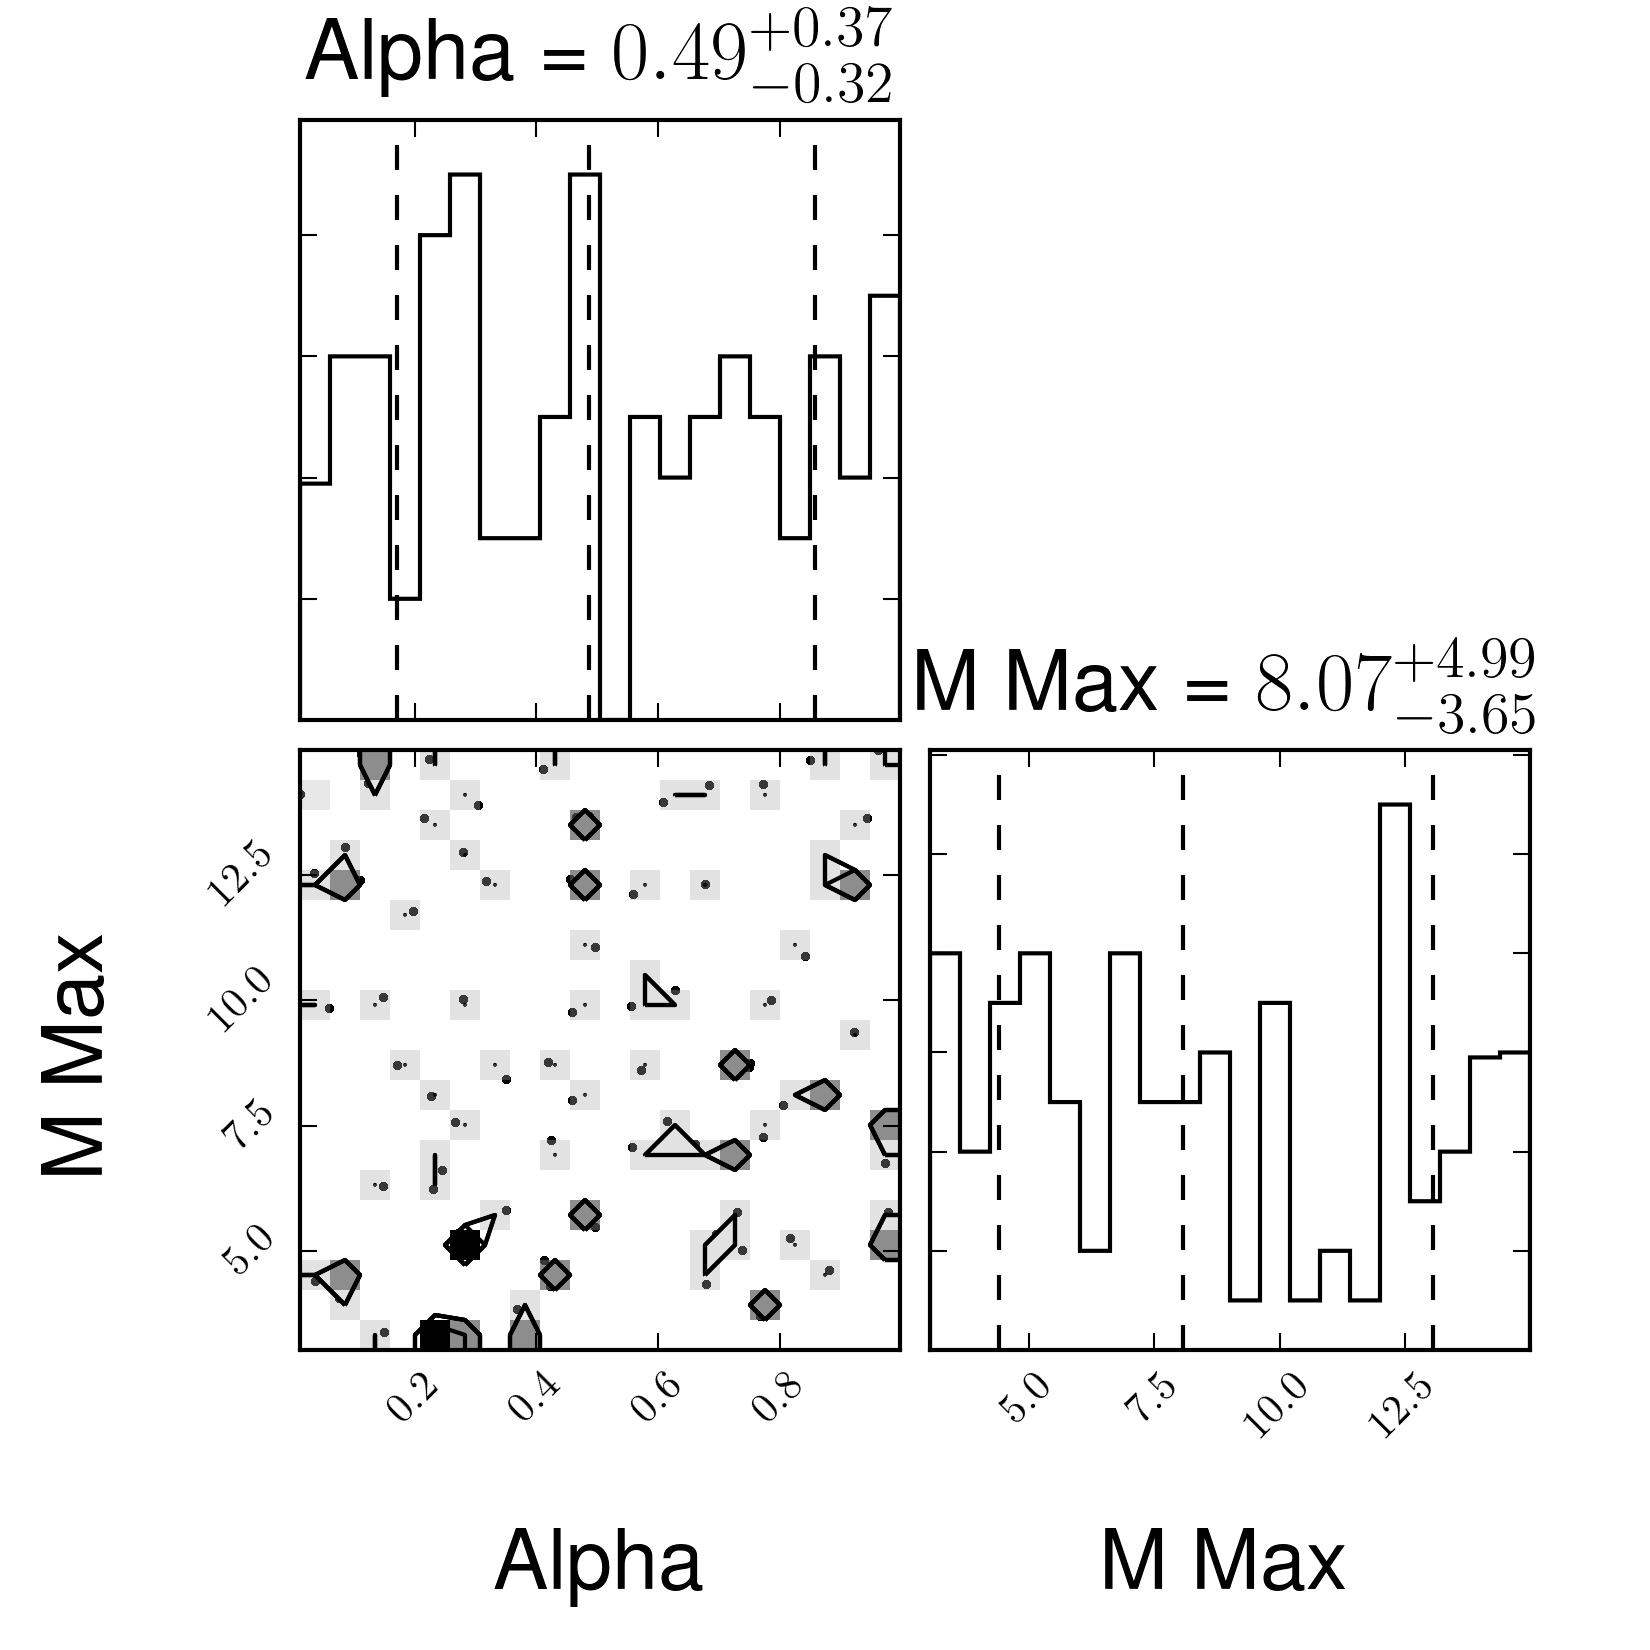
\includegraphics[scale = 0.6]{corner_plot_emcee_prob2_10_data.png}
%\end{figure}

\begin{figure}[H]
\caption{These figures are from a 10 mass point data set.}
\centering
\begin{subfigure}{.4\textwidth}
  \centering
  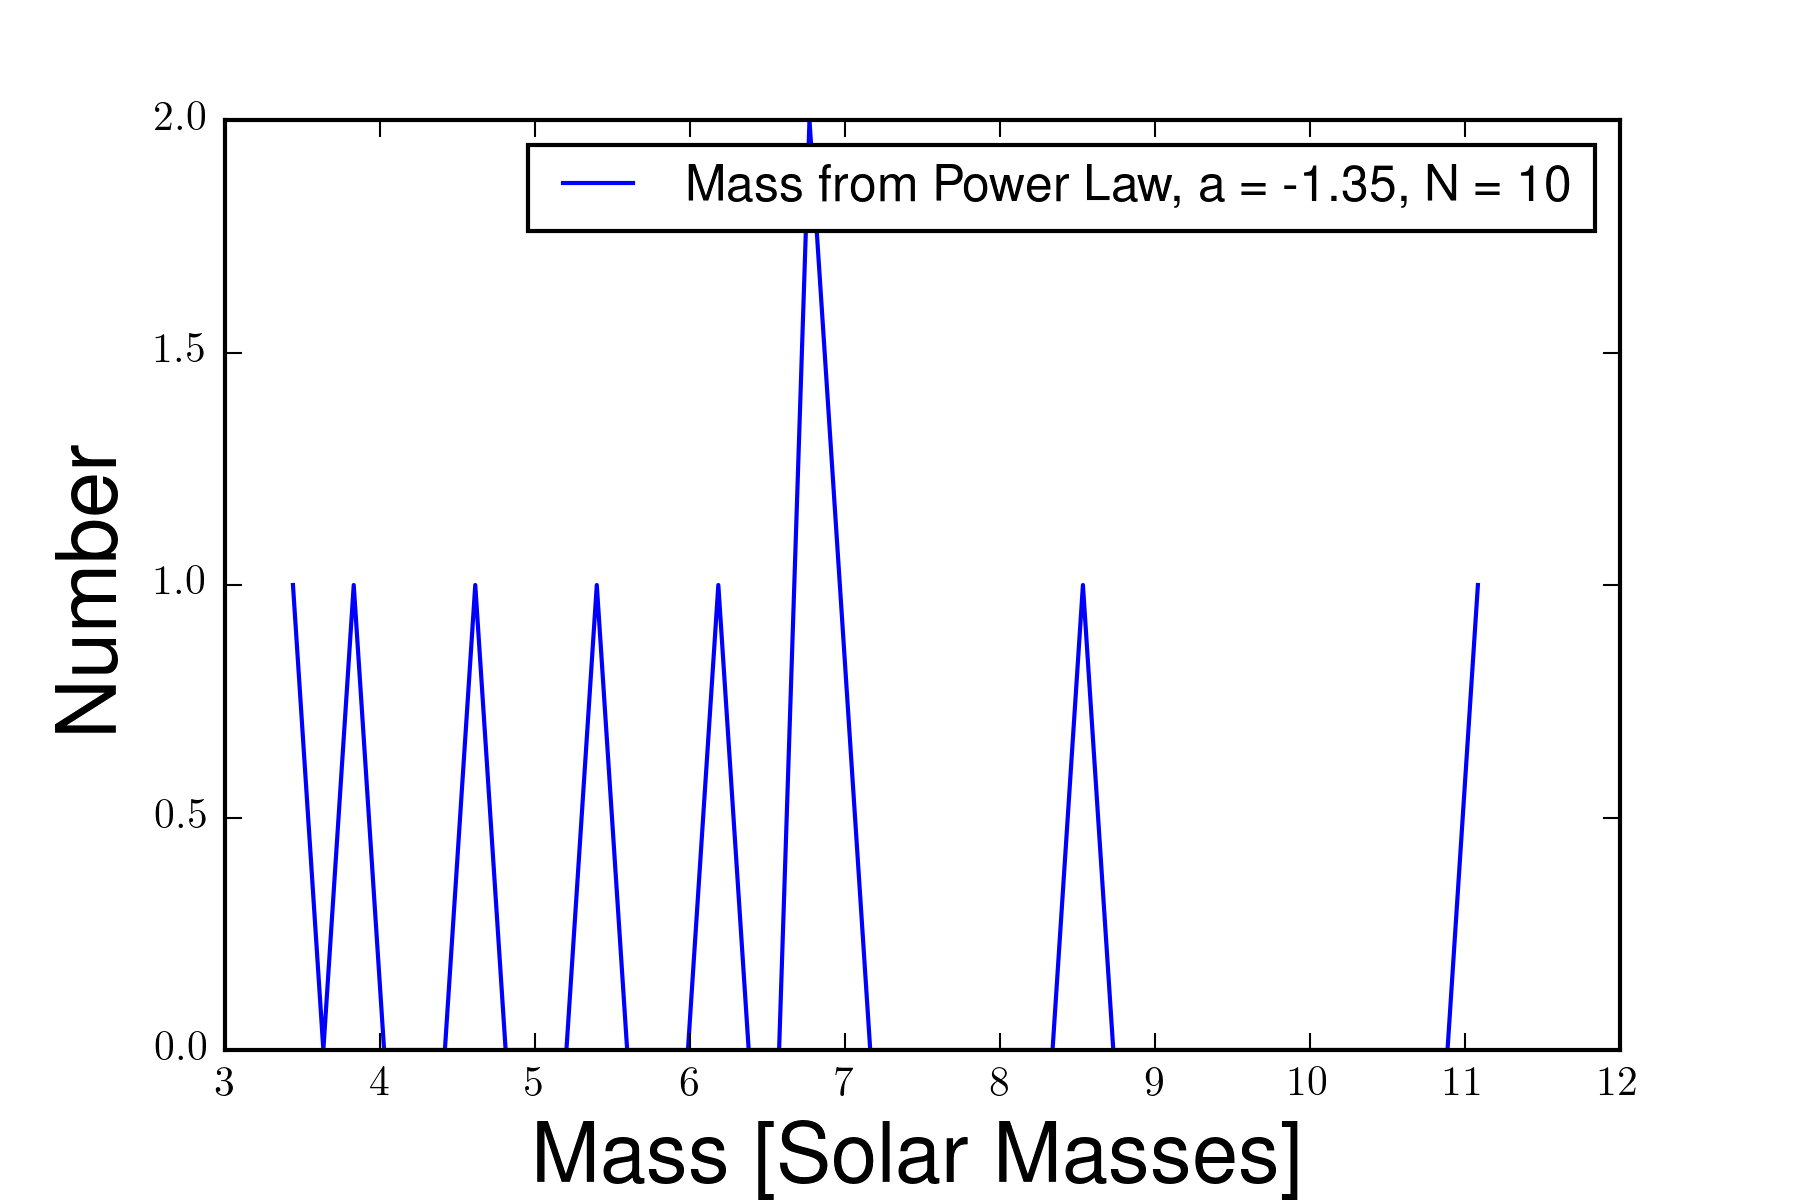
\includegraphics[width=\linewidth]{mass_histogram_prob2_10_data.png}
  \caption{Mass Histogram}
  \label{fig:sub1x}
\end{subfigure}%
\begin{subfigure}{0.4\textwidth}
  \centering
  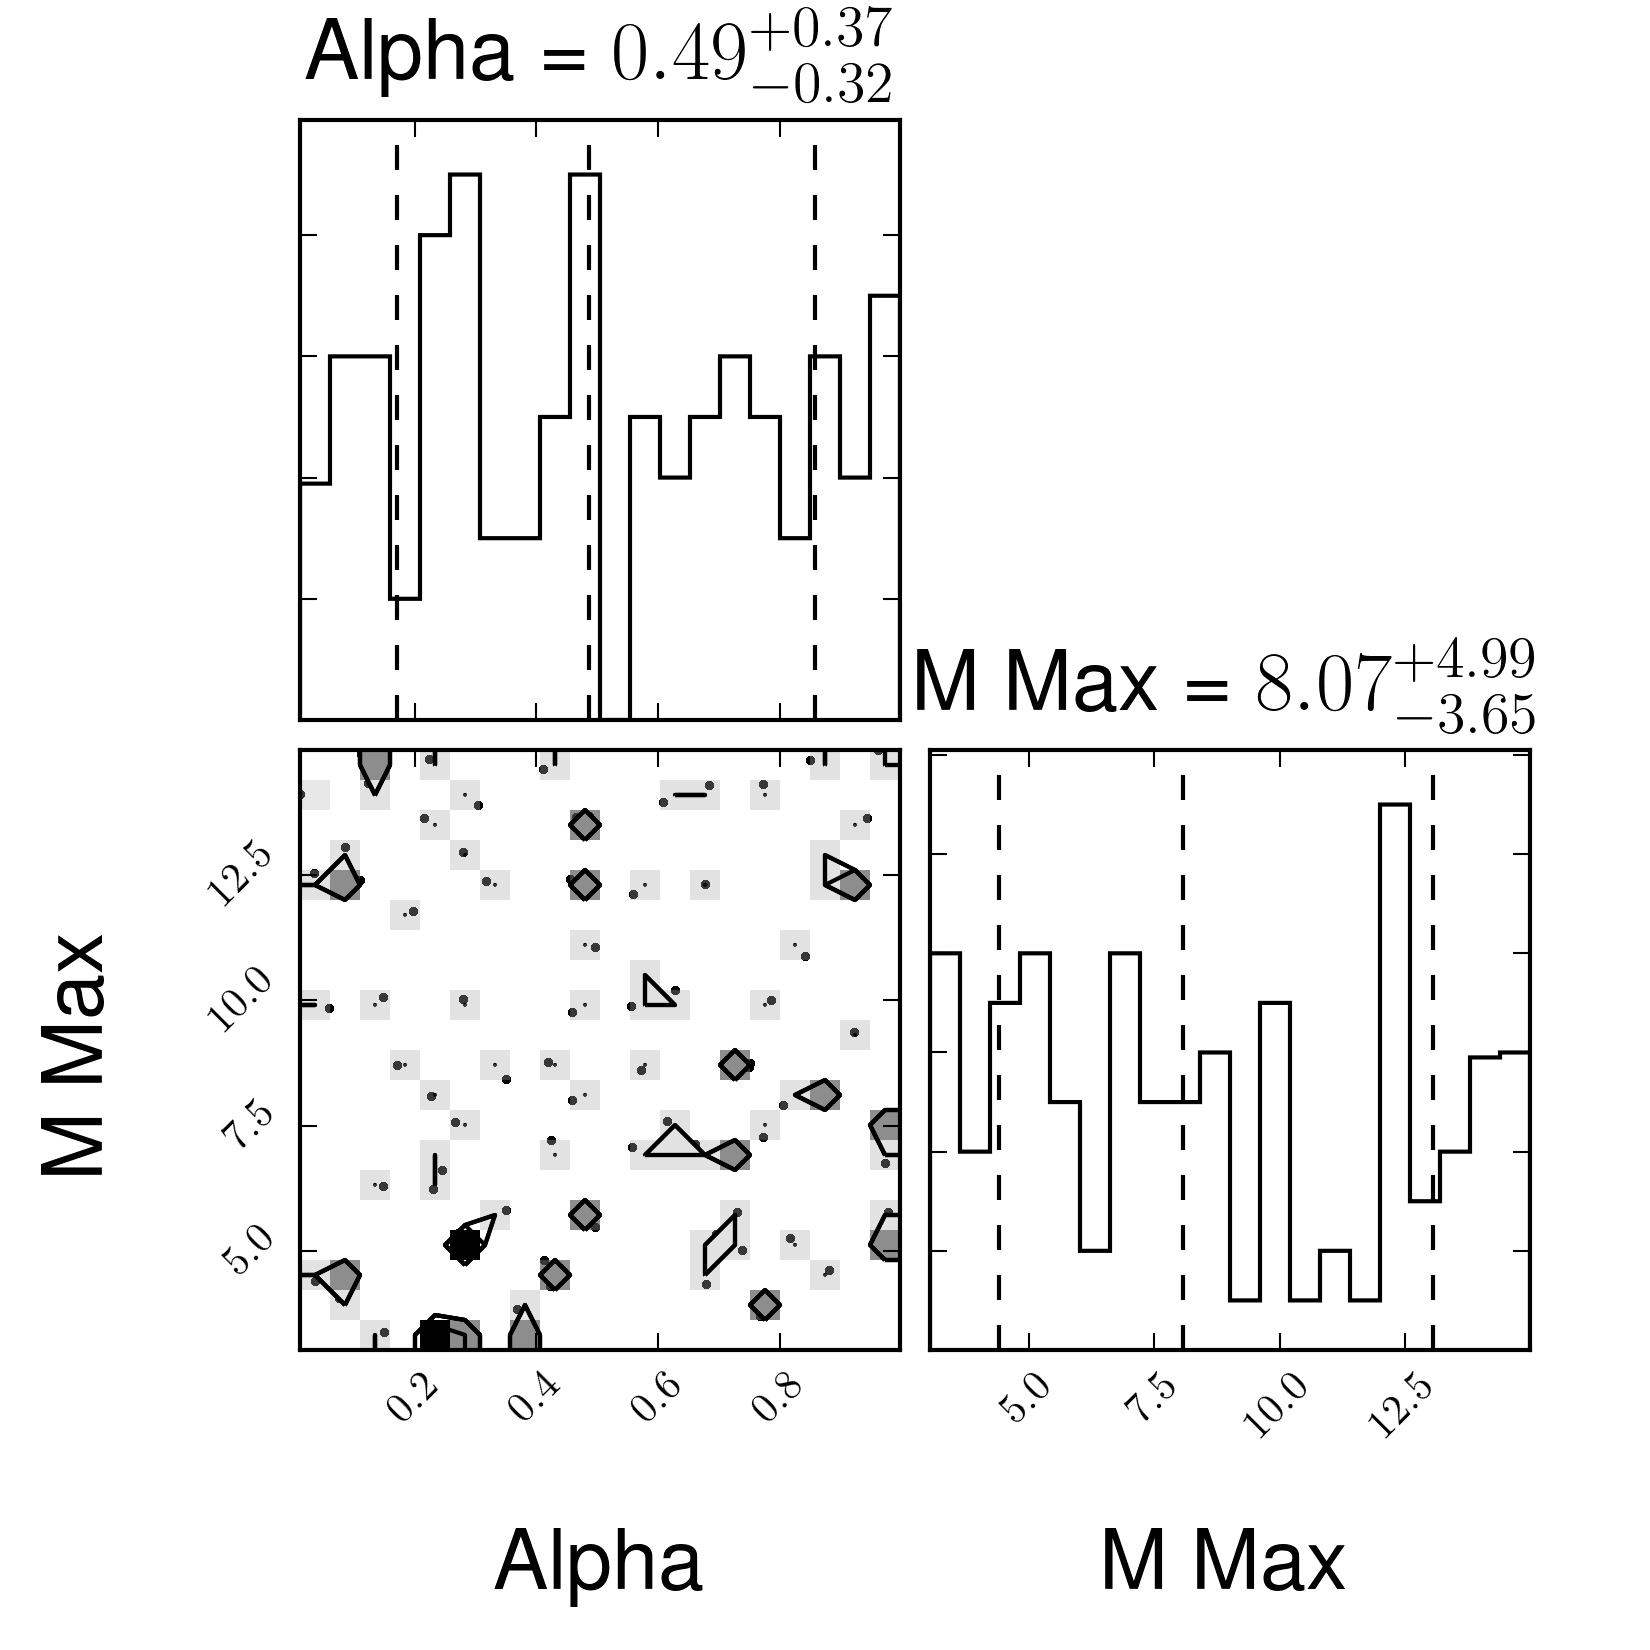
\includegraphics[width=\linewidth]{corner_plot_emcee_prob2_10_data.png}
  \caption{Contour Plot}
  \label{fig:sub2x}
\end{subfigure}
\label{fig:testx}
\end{figure}

\begin{figure}[H]
\caption{These figures are from a 100 mass point data set.}
\centering
\begin{subfigure}{.4\textwidth}
  \centering
  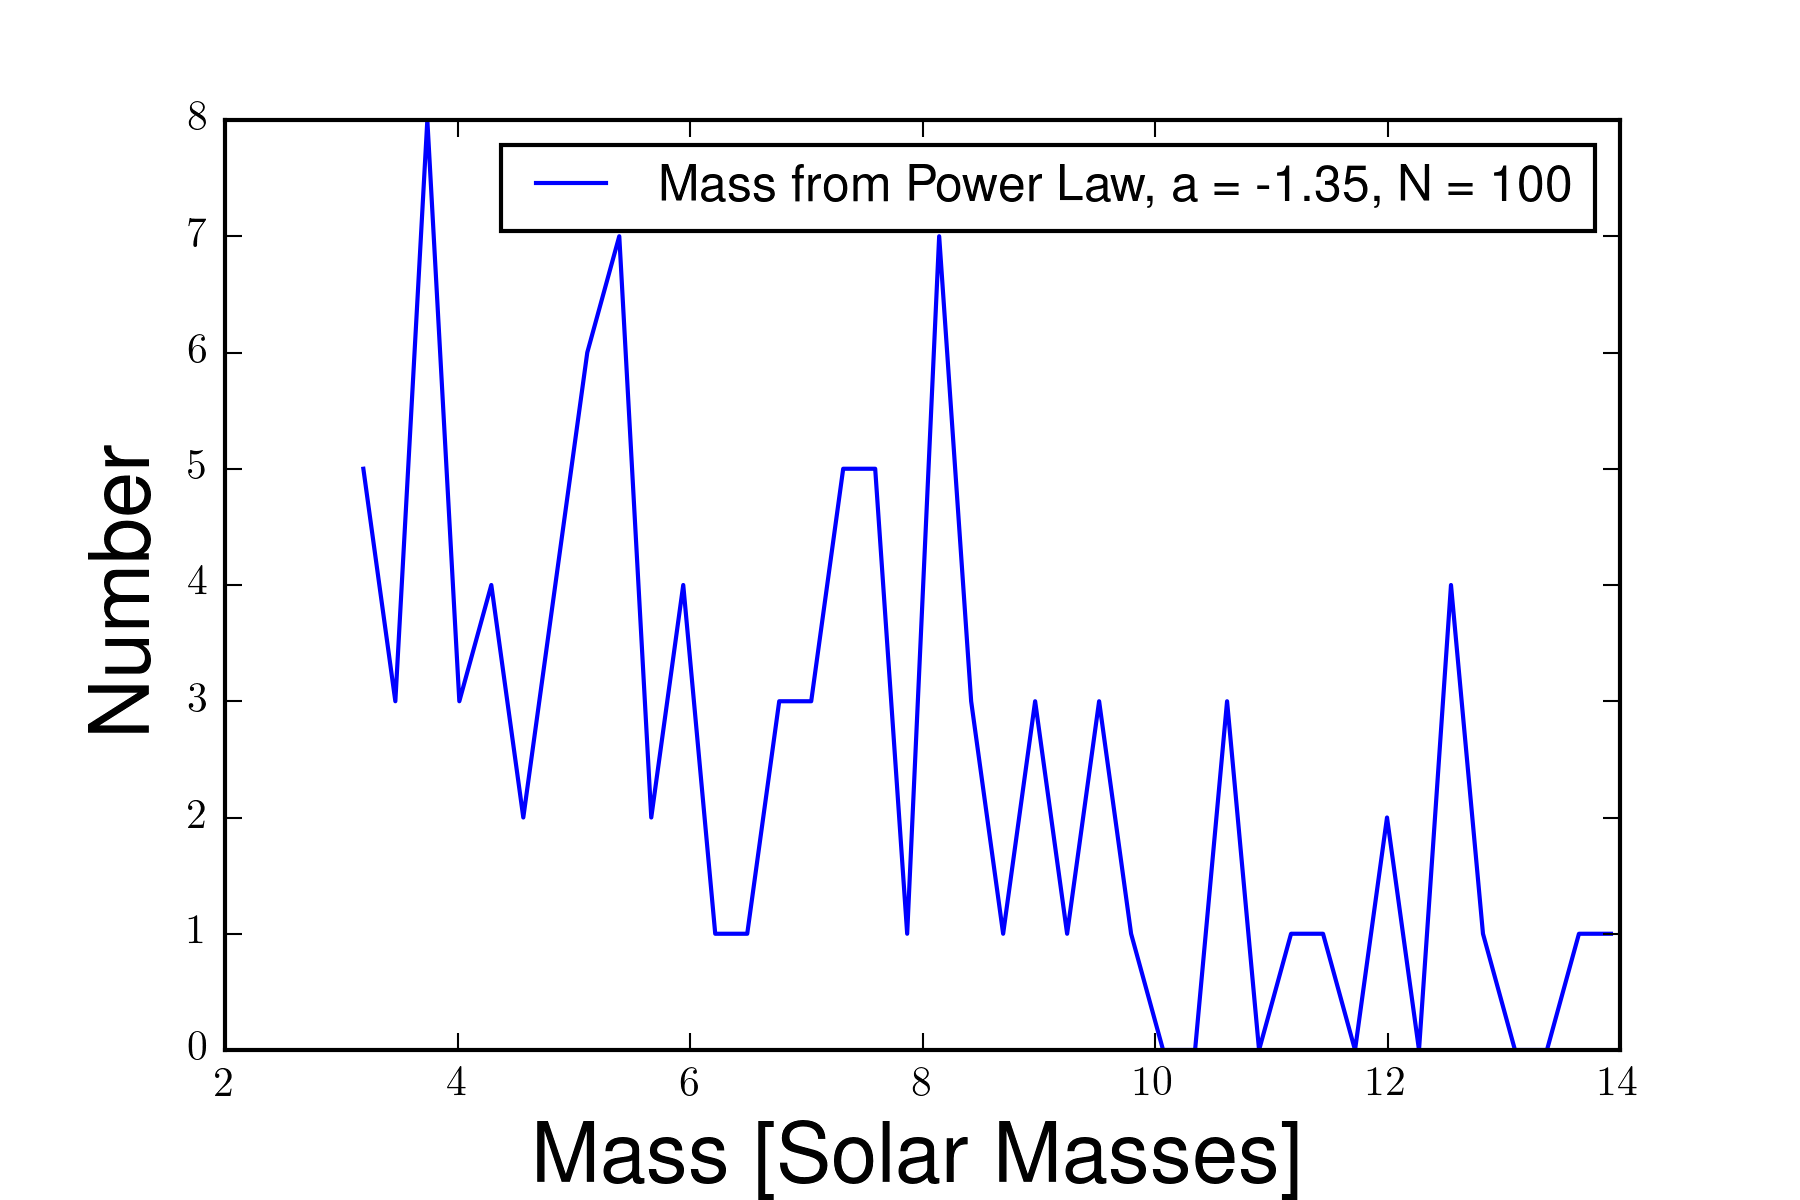
\includegraphics[width=\linewidth]{mass_histogram_prob2_100_data.png}
  \caption{Mass Histogram}
  \label{fig:sub1x}
\end{subfigure}%
\begin{subfigure}{0.4\textwidth}
  \centering
  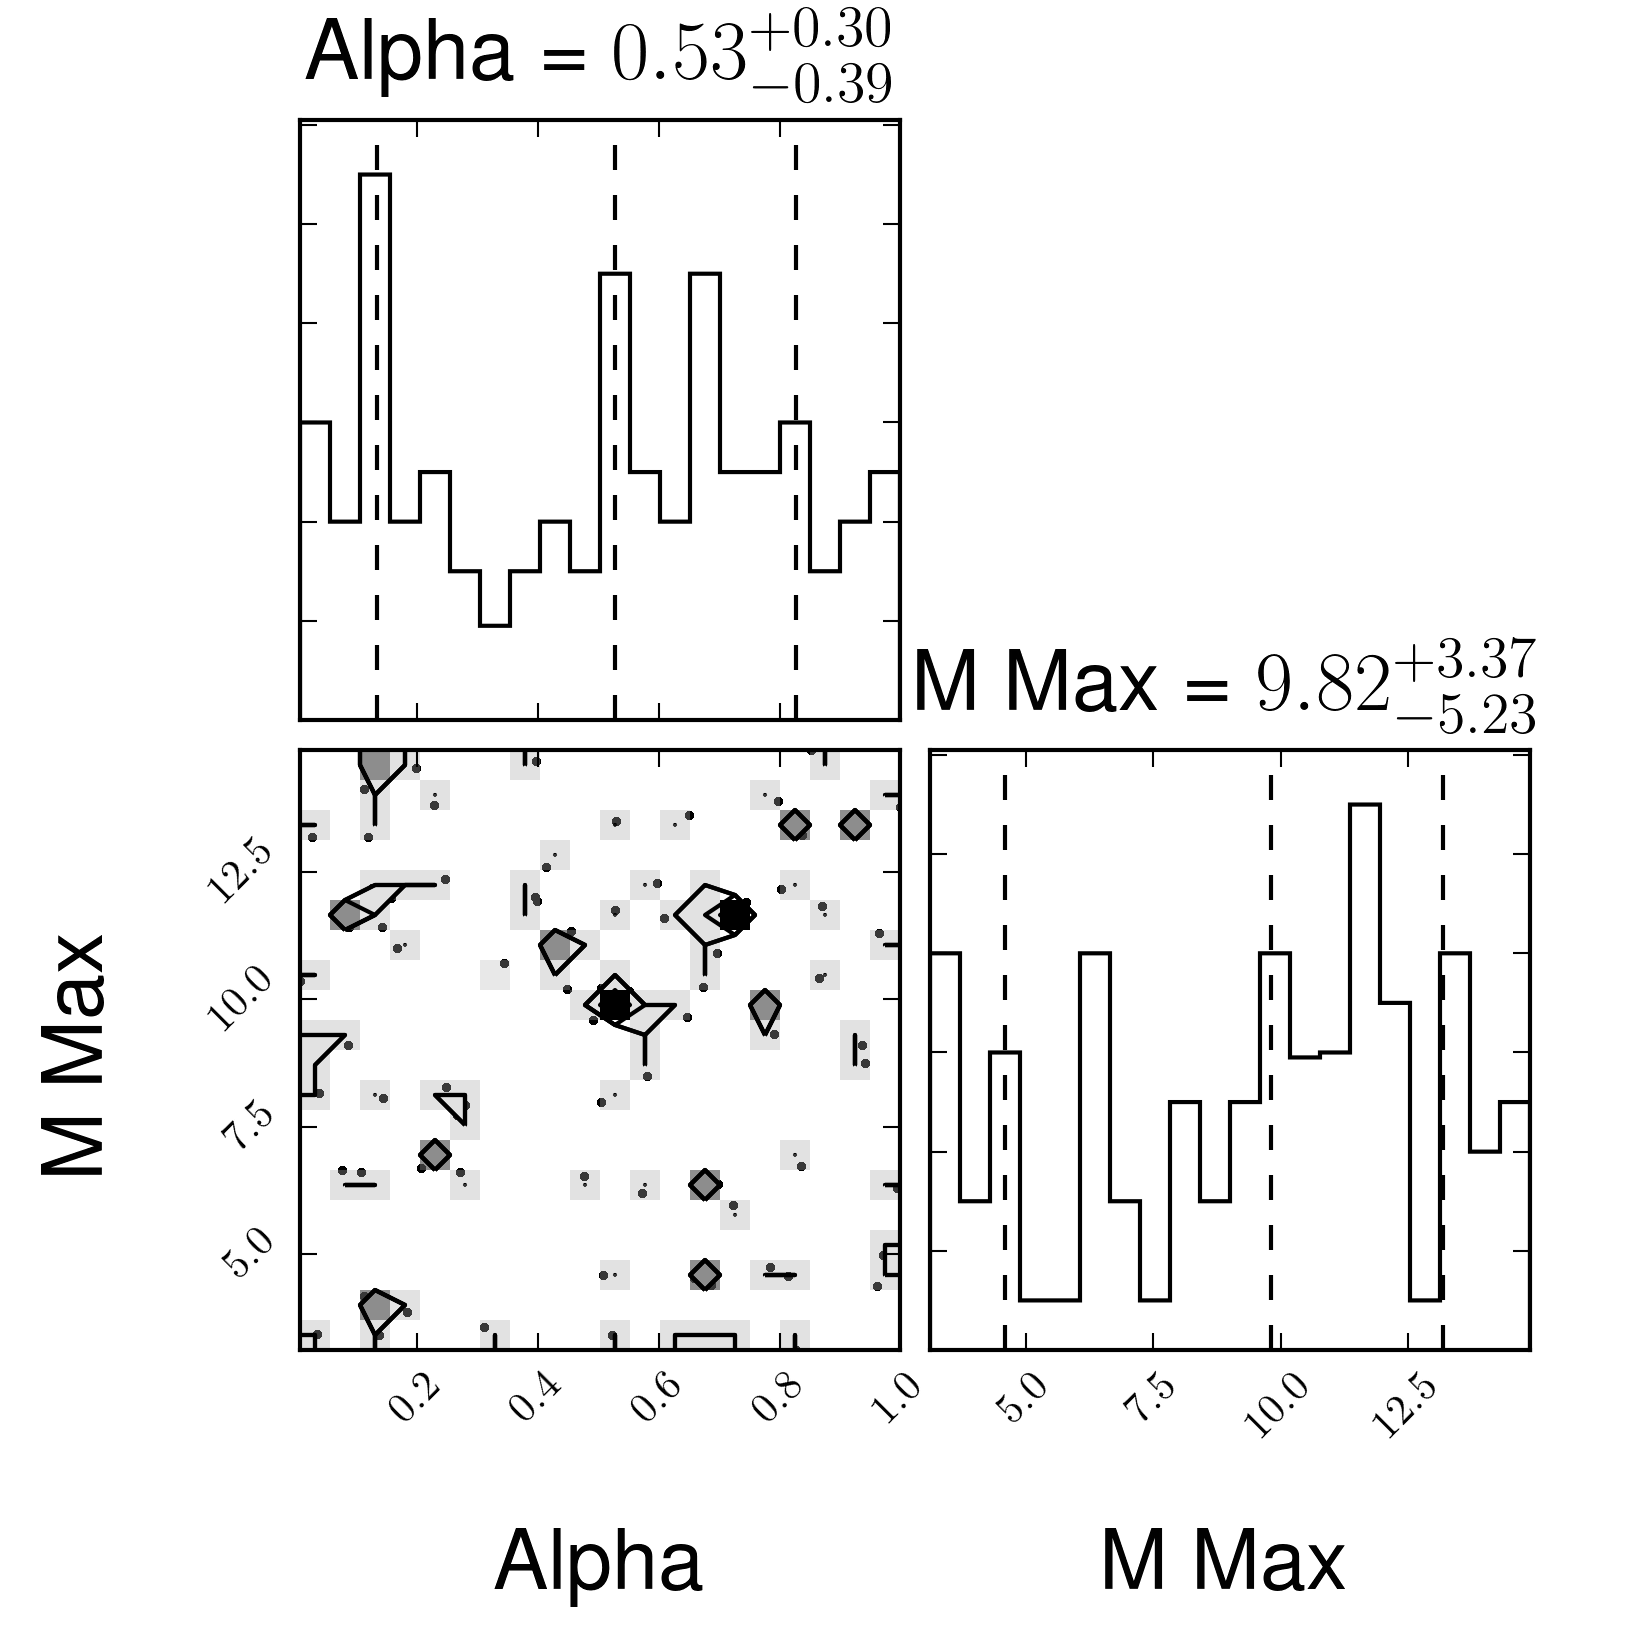
\includegraphics[width=\linewidth]{corner_plot_emcee_prob2_100_data.png}
  \caption{Contour Plot}
  \label{fig:sub2x}
\end{subfigure}
\label{fig:testx}
\end{figure}

\begin{figure}[H]
\caption{These figures are from a 1,000 mass point data set.}
\centering
\begin{subfigure}{.4\textwidth}
  \centering
  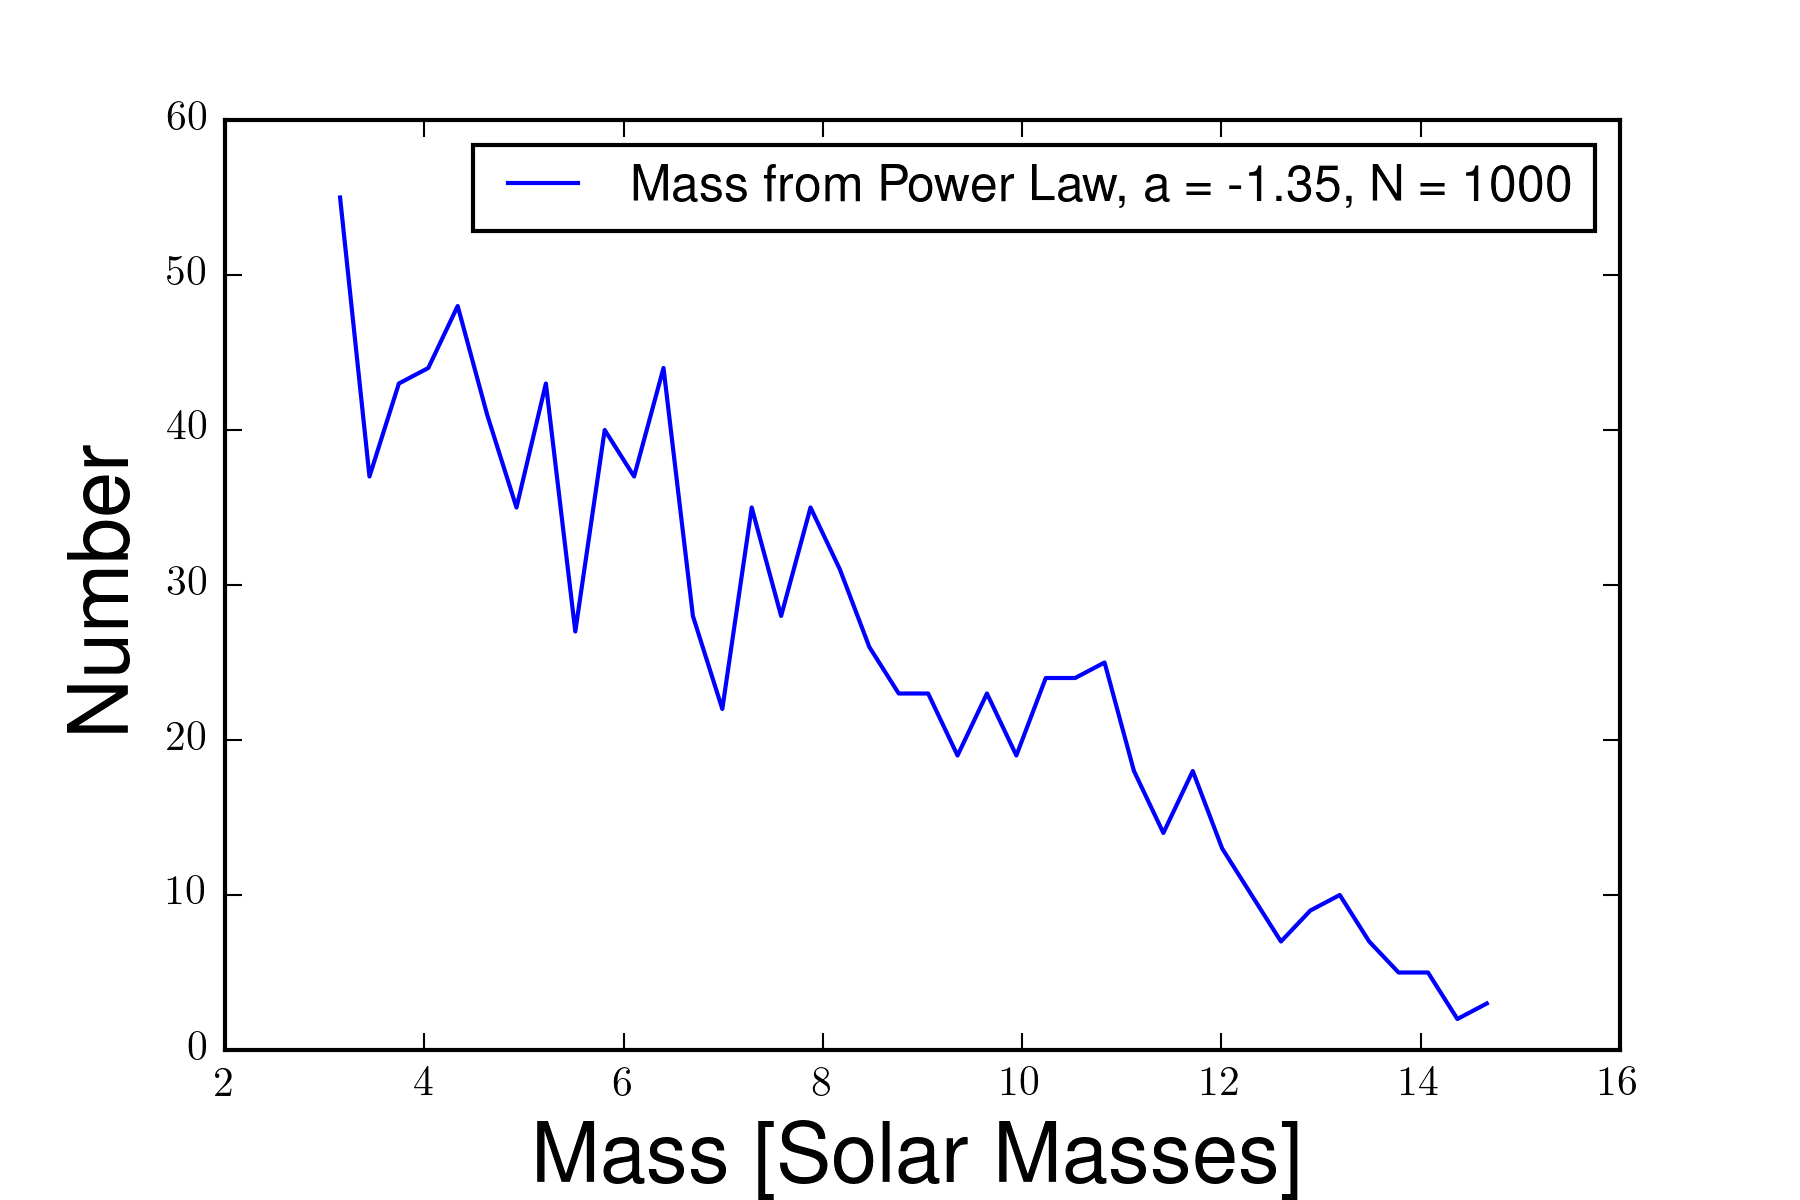
\includegraphics[width=\linewidth]{mass_histogram_prob2_1000_data.png}
  \caption{Mass Histogram}
  \label{fig:sub1x}
\end{subfigure}%
\begin{subfigure}{0.4\textwidth}
  \centering
  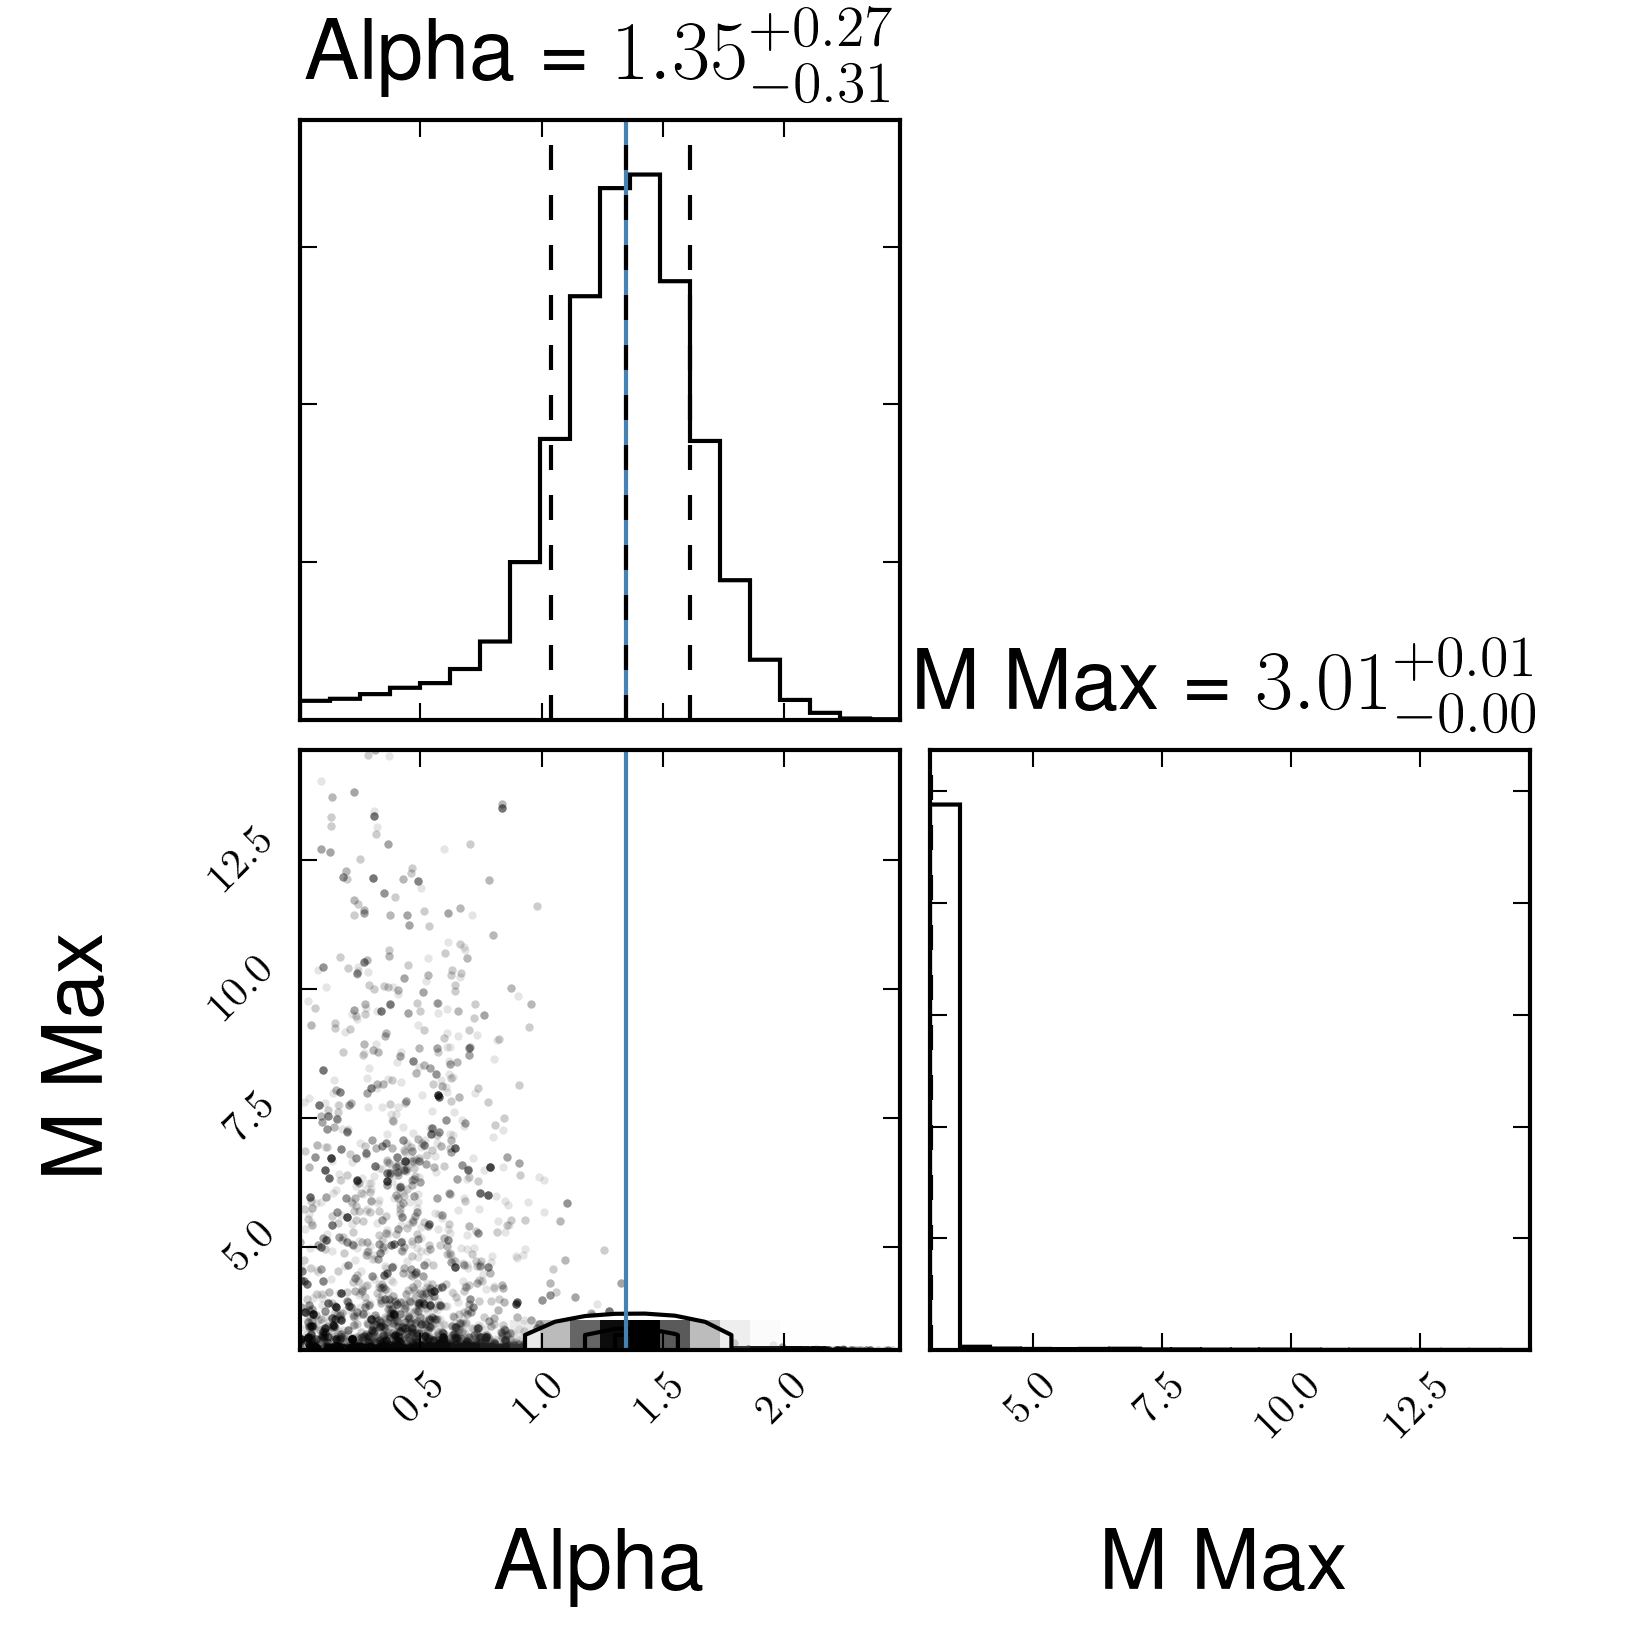
\includegraphics[width=\linewidth]{corner_plot_emcee_prob2_1000_data.png}
  \caption{Contour Plot}
  \label{fig:sub2x}
\end{subfigure}
\label{fig:testx}
\end{figure}

\begin{figure}[H]
\caption{These figures are from a 10,000 mass point data set.}
\centering
\begin{subfigure}{.4\textwidth}
  \centering
  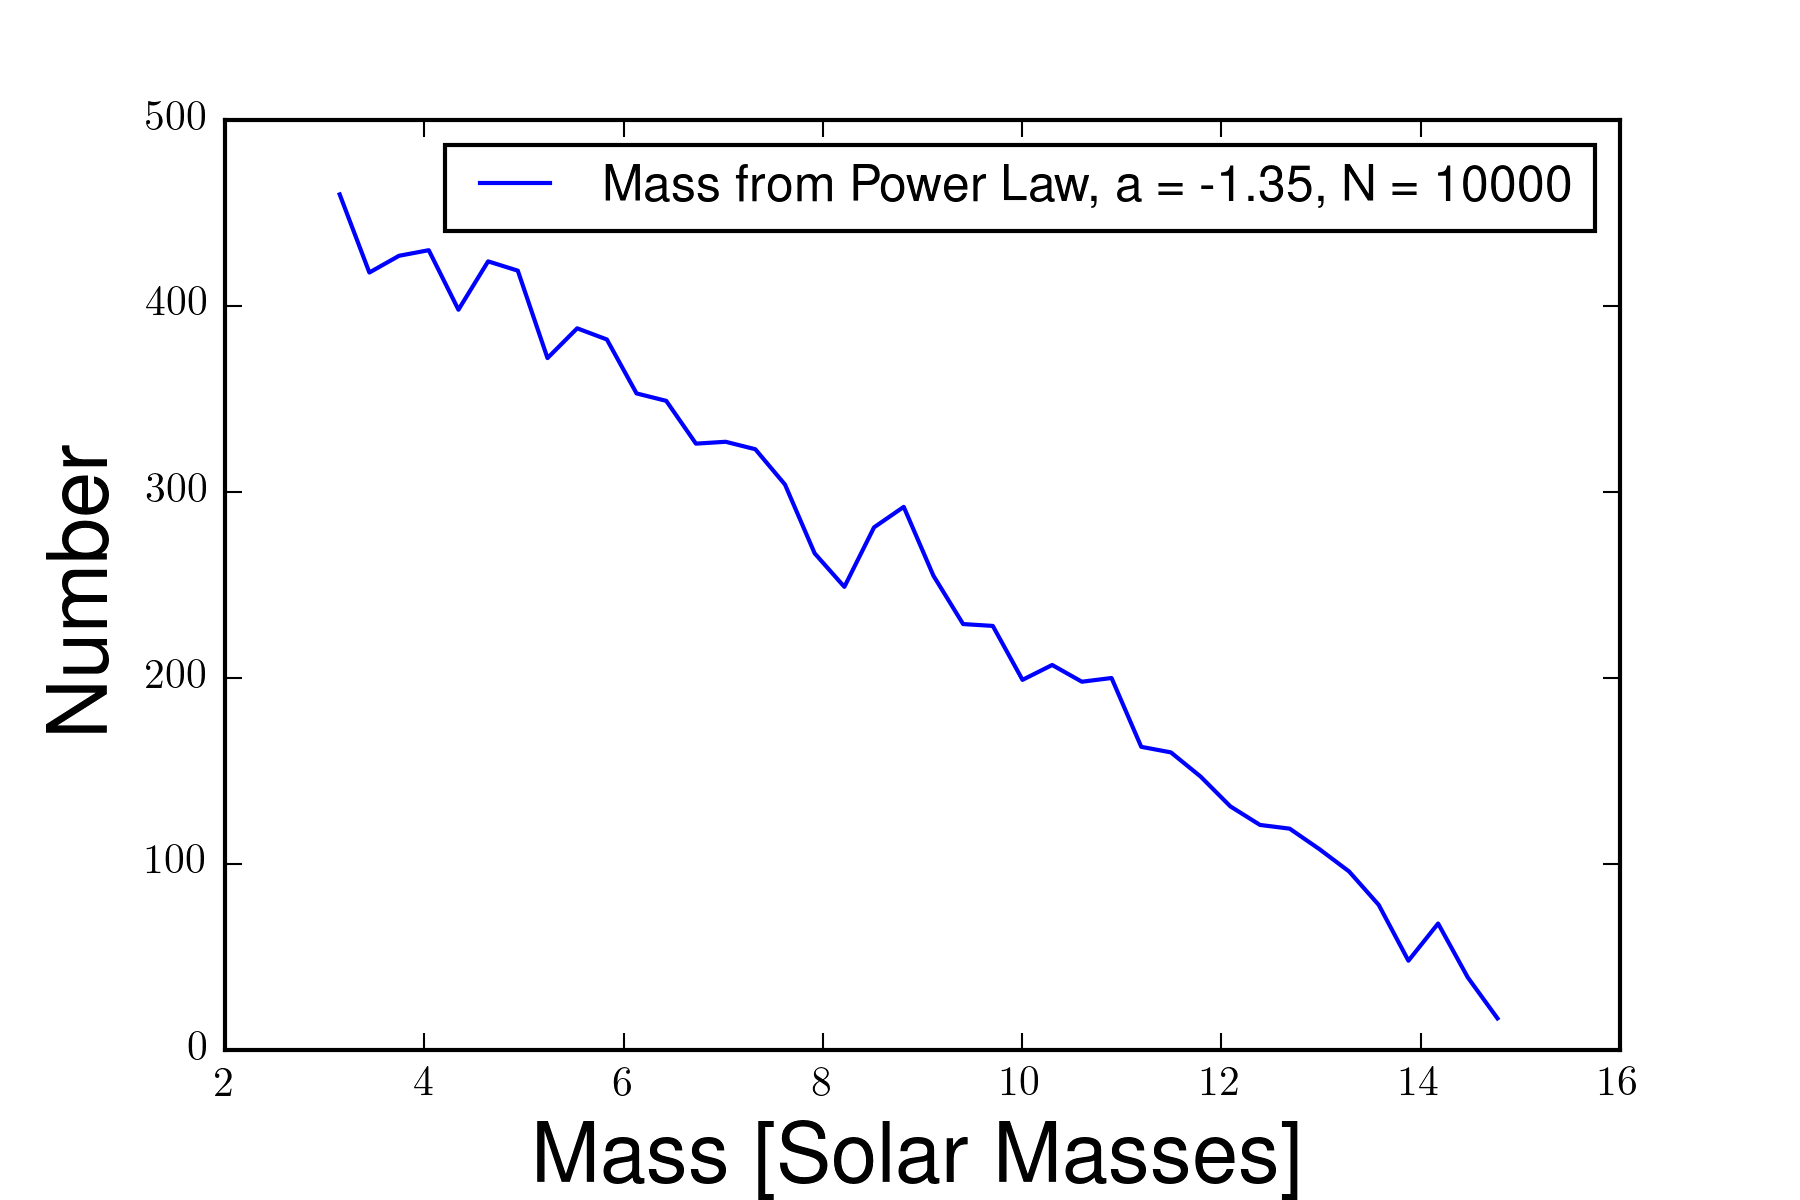
\includegraphics[width=\linewidth]{mass_histogram_prob2_10000_data.png}
  \caption{Mass Histogram}
  \label{fig:sub1x}
\end{subfigure}%
\begin{subfigure}{0.4\textwidth}
  \centering
  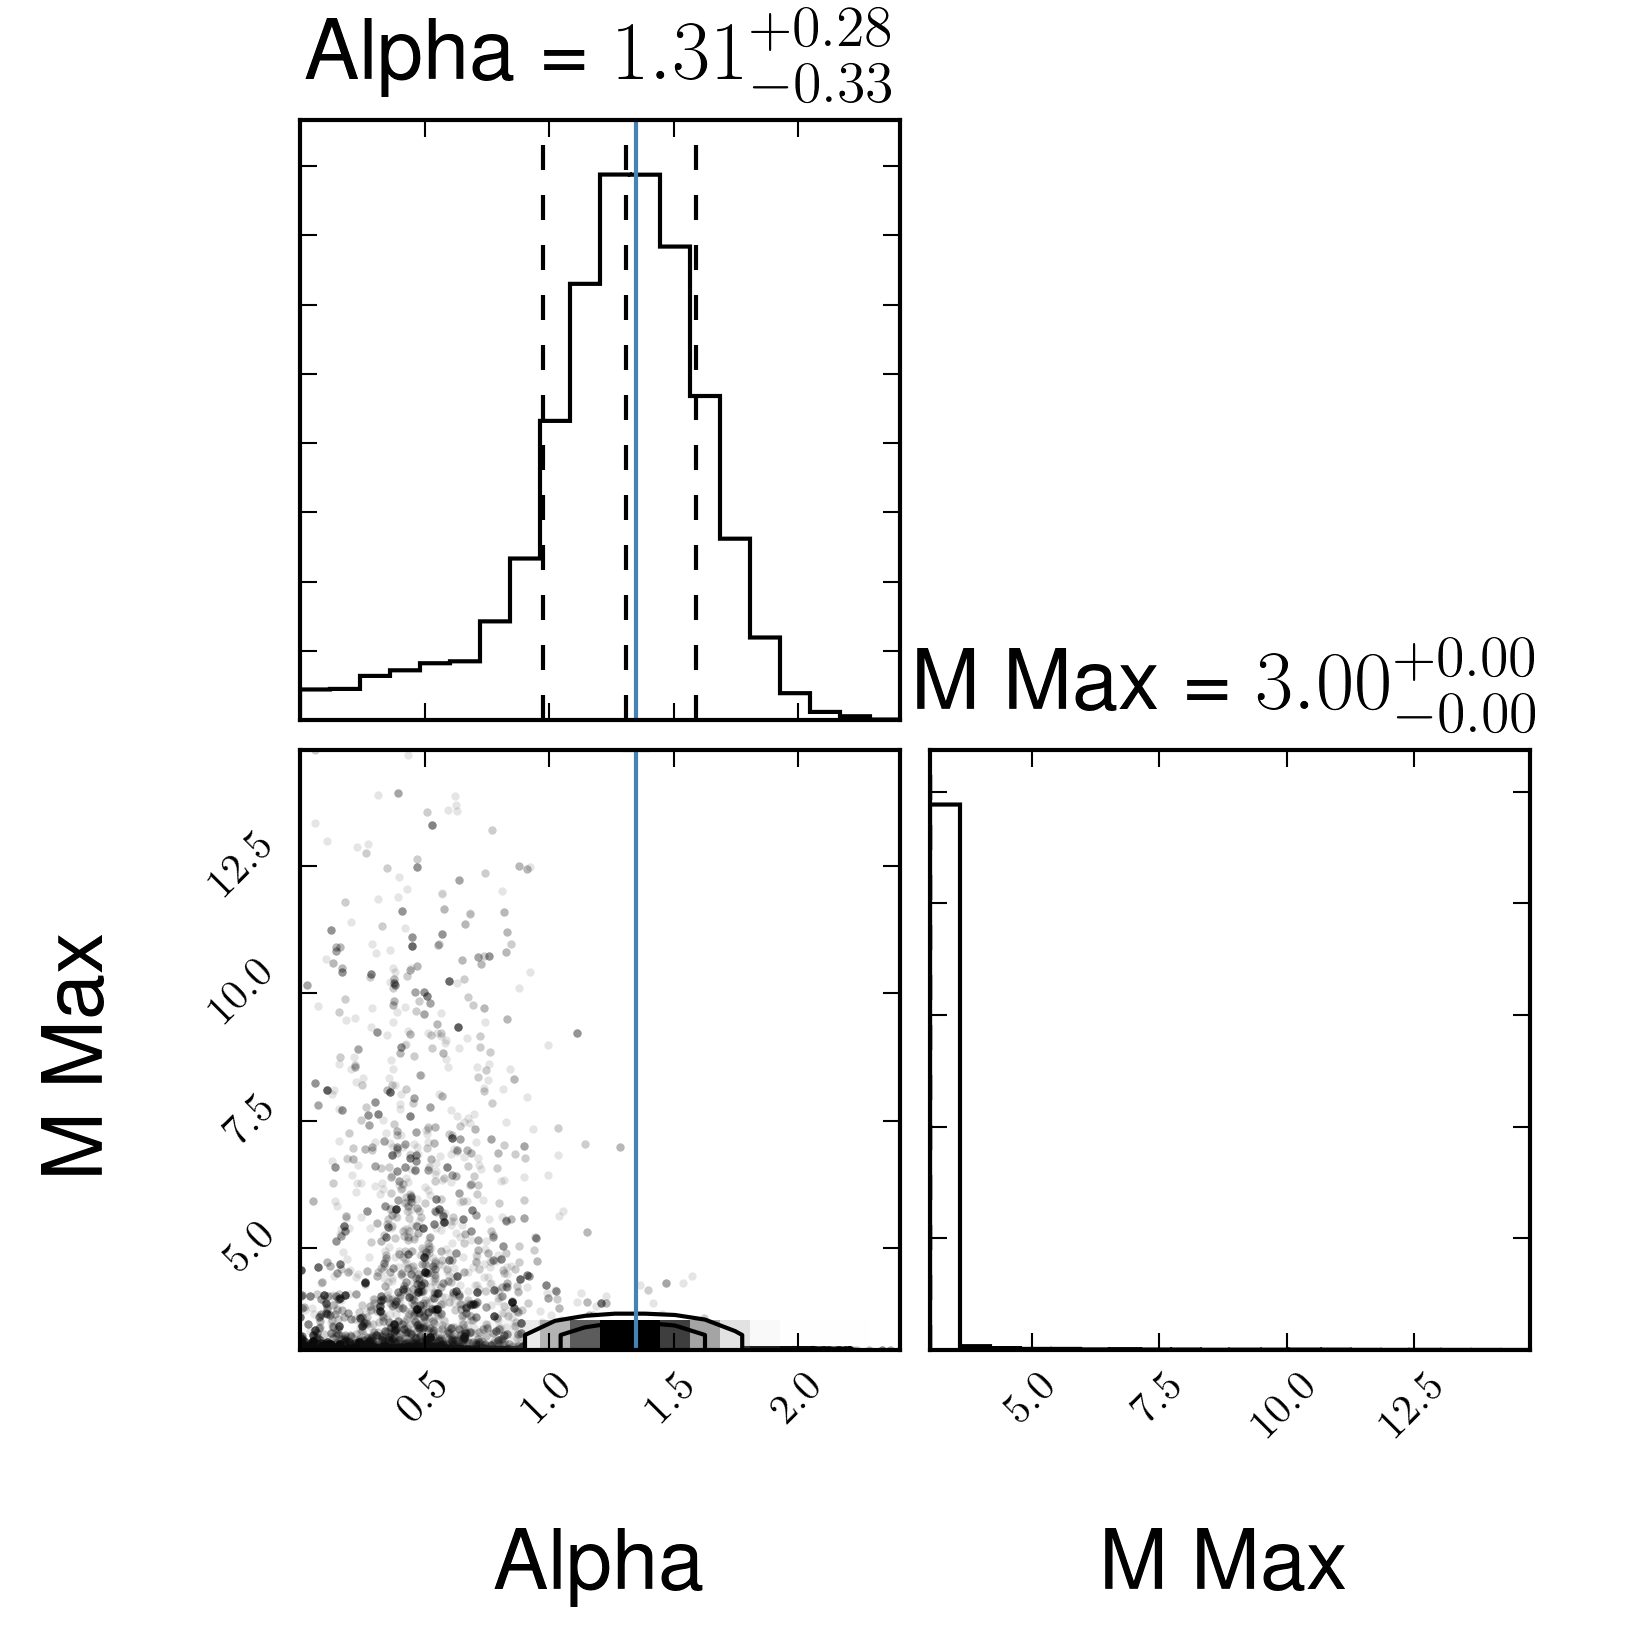
\includegraphics[width=\linewidth]{corner_plot_emcee_prob2_10000_data.png}
  \caption{Contour Plot}
  \label{fig:sub2x}
\end{subfigure}
\label{fig:testx}
\end{figure}

Data set size clearly plays a large role in the accuracy of the measurement. In very small data sets, the histogram method fails because there aren't enough data points to have a well populated histogram. Although I don't think this problem can be completely avoided using another method since 10 data points is inherently limiting. Additionally, the least amount of variation seemed to arise in the N = 1,000 sample size. Oddly, the 10,000 star sample varied from run to run more than for 1,000.

\section*{Problem 3}
\textit{In this problem, we will attempt to re-create Salpeter's original IMF measurement.}\\
The code for this problem is contained in the file \textbf{ps2\_problem3.ipynb}.

\subsection*{(a)}
\textit{Using the data for mass and number density in Table 2 and/or Figure 2 in Salpeter (1955), fit a power-law using an optimizer or least squares fitter (e.g., scipy.optimize).}

For this problem I used the function scipy.optimize.least\_squares to fit a power law to the data from the Salpeter 1955 paper. This yielded a slope of 1.407 and a normalization constant of 0.036. Below is a plot of the original data from the paper, plotted with the least squares fit. By inspection, the fit seems to agree with the data.

\begin{figure}[H]
\centering
\caption{Salpeter 1955 data and the Least Squares Fit}
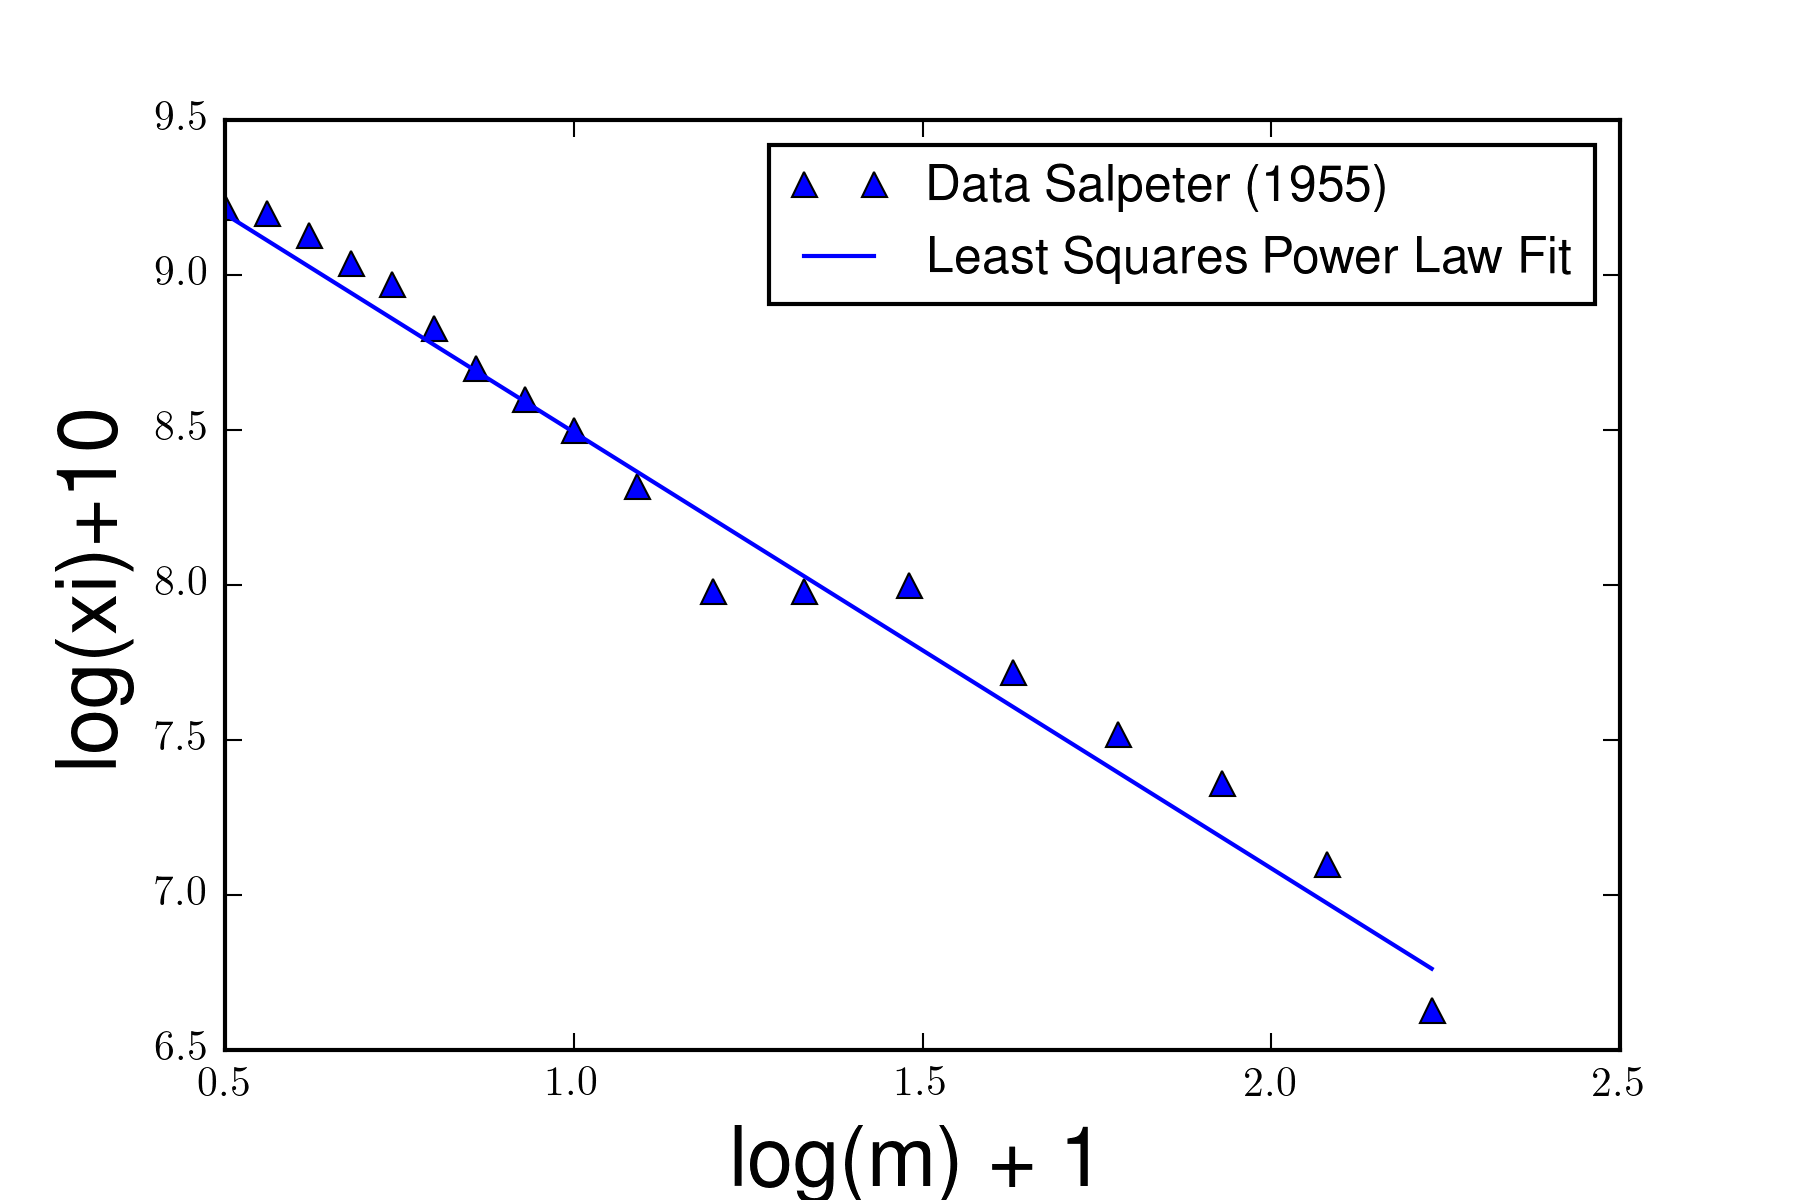
\includegraphics[scale = 0.6]{least_squares_fit_prob_3.png}
\end{figure}

\subsection*{(b)}
\textit{Same as part (a) only using your own inference code and emcee. Compare the two results: How close are they to one another? How close are they to the value reported in Salpeter(1955)?}\\
For this part of the problem I used emcee to fit both the slope of the power law and the normalization constant.

\begin{figure}[H]
\caption{Emcee $\alpha$ and Normalization Constant vs. Step Number}
\centering
\begin{subfigure}{.4\textwidth}
  \centering
  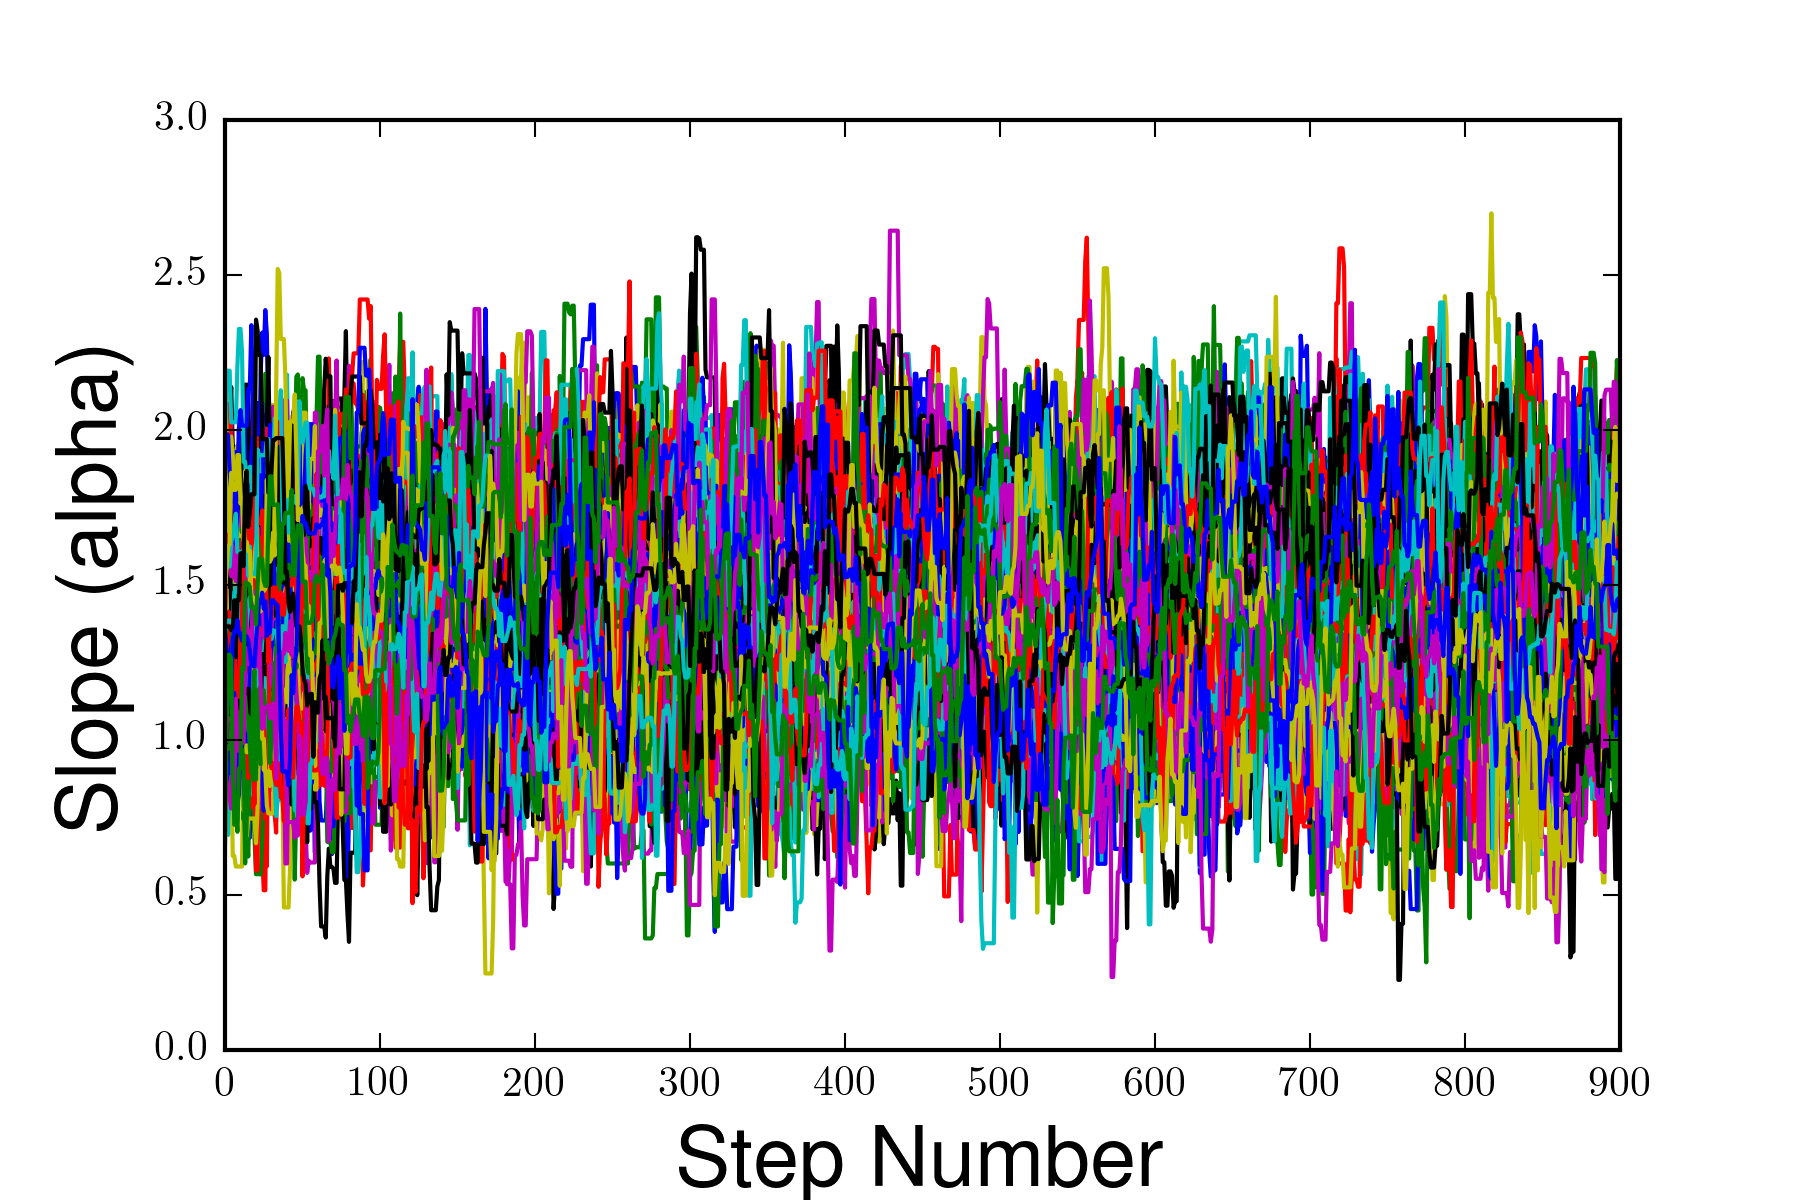
\includegraphics[width=\linewidth]{m_step_emcee_prob3.png}
  \caption{}
  \label{fig:sub1x}
\end{subfigure}%
\begin{subfigure}{0.4\textwidth}
  \centering
  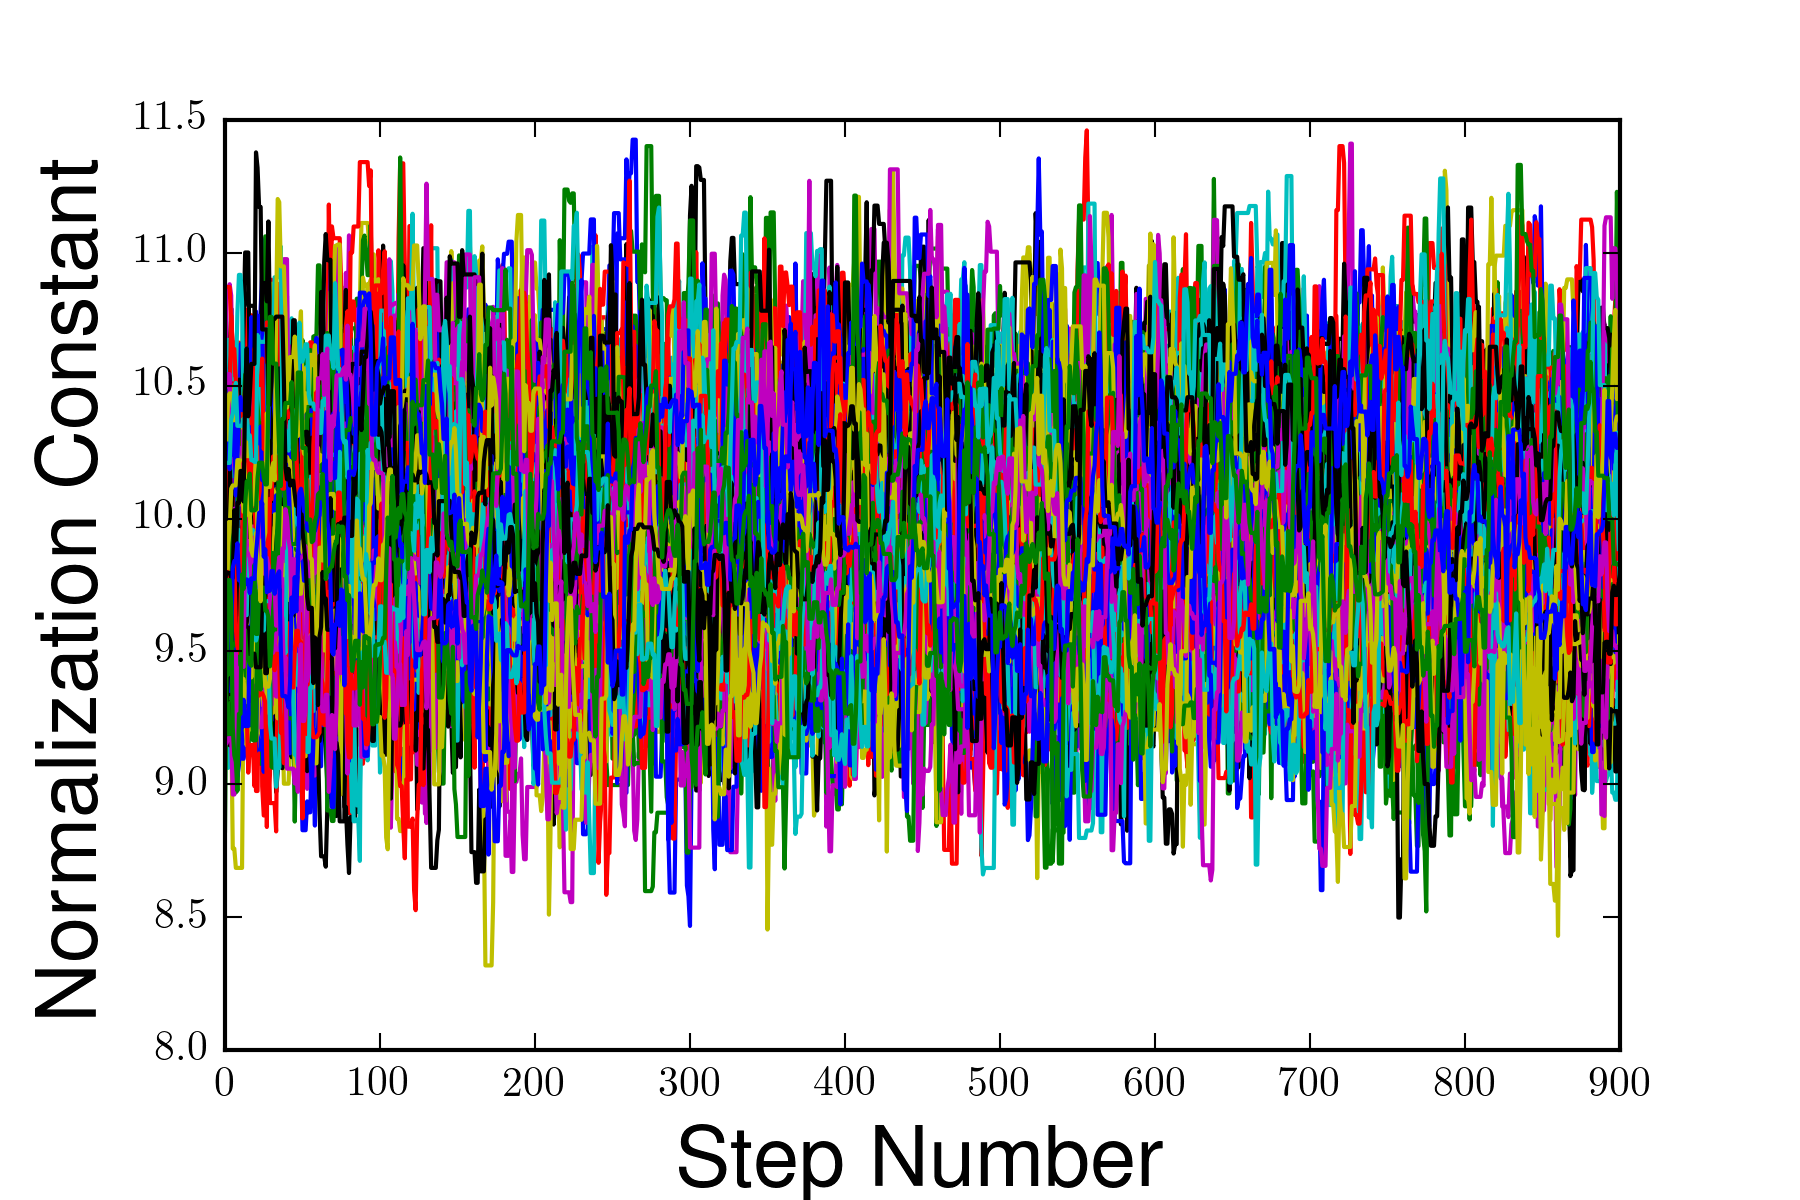
\includegraphics[width=\linewidth]{const_step_emcee_prob3.png}
  \caption{}
  \label{fig:sub2x}
\end{subfigure}
\label{fig:testx}
\end{figure}


\begin{figure}[H]
\centering
\caption{Salpeter 1955 data and the Least Squares Fit}
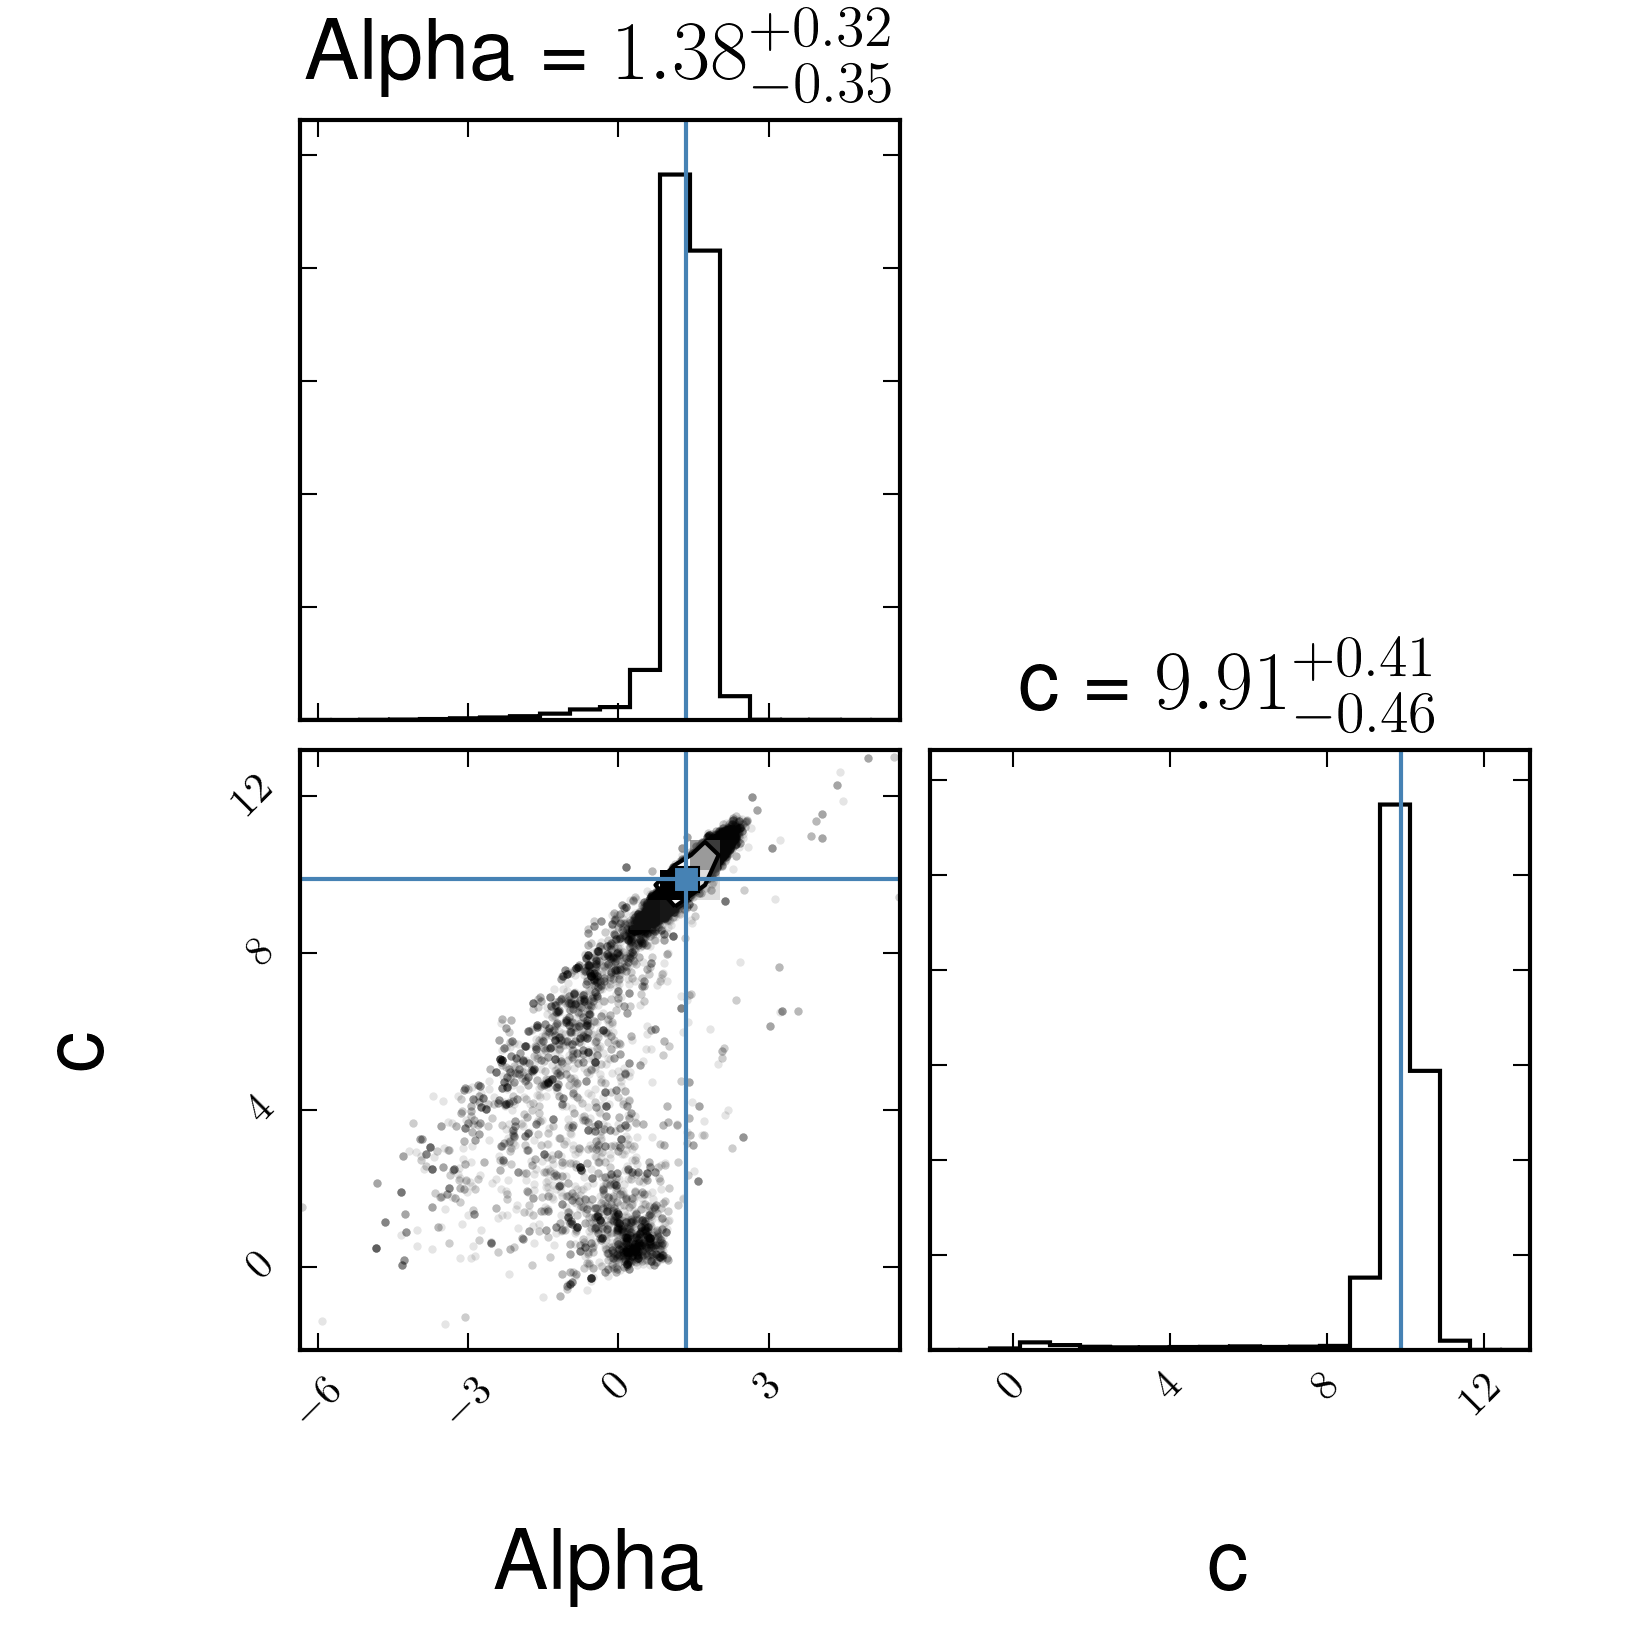
\includegraphics[scale = 0.6]{corner_plot_emcee_prob3.png}
\end{figure}

Below is a plot of the three slope values: Salpeter's original fit, the least squares scipy.optimize fit and the emcee fit.
\begin{figure}[H]
\centering
\caption{Data with the three different fits}
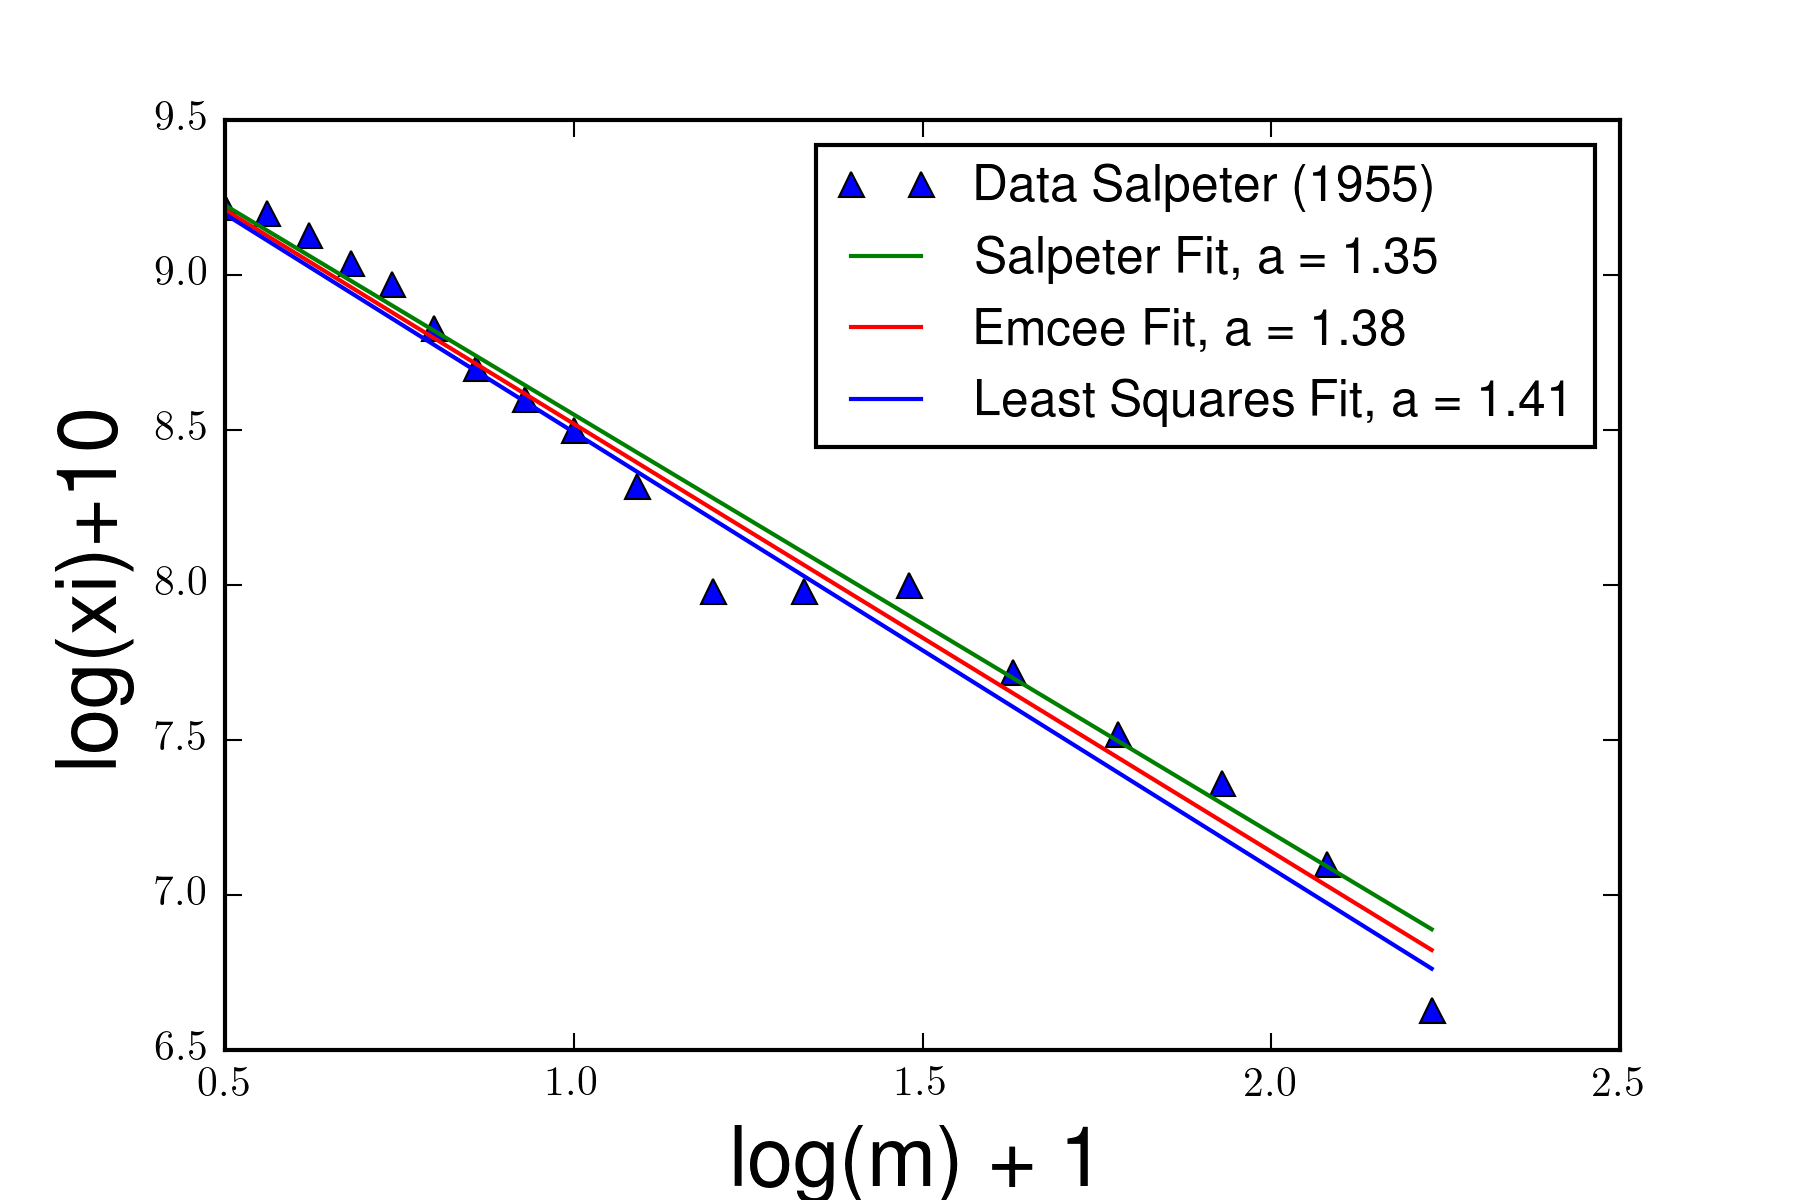
\includegraphics[scale = 0.8]{fit_comparison_power_law_prob3.png}
\end{figure}
While the values are all fairly close, there are small differences. One reason Salpeter's curve may diverge from my measured values is that he threw away the three points in the center of the data that show a flat trend.

\section*{Problem 4}
\textit{There are claims in the literature that low-mass IMF slope may systematically deviate from the Galactic value in low-mass dwarf galaxies. However, these measurements are made over a fairly limited mass range (usually $\approx$ 0.5-0.8 $M_{\odot}$) and done so assuming that a power-law is a reasonable approximation for the low-mass IMF.
Suppose the true IMF for stars with M $<$ $1 M_{\odot}$ in all galaxies is actually a Chabrier IMF, i.e., a log-normal at low masses. Ignoring corrections for stellar multiplicity, this IMF has the functional form:}

\begin{equation}
\xi (m) \Delta m = \frac{0.15}{m}exp \frac{-(log(m) - log(0.08))^2}{(2 \times 0.69^2)}
\end{equation}

The code for this problem is available in the file \textbf{ps2\_problem4.ipynb}.
\subsection*{(a)}
\textit{Using the Chabrier IMF from above, generate a list of N = 10,000 (perfectly-known) stellar masses between 0.5 and 0.8 $M_{\odot}$.}
For this problem, I used emcee to sample the Chabrier IMF using the functional form as the likelihood function. The prior I used forced the masses to be within the specified mass range.
Below is a plot demonstrating the sampled masses plotted with the analytic function.

\begin{figure}[H]
\centering
\caption{Mass sample of 10,000 stars from Chabrier Distribution}
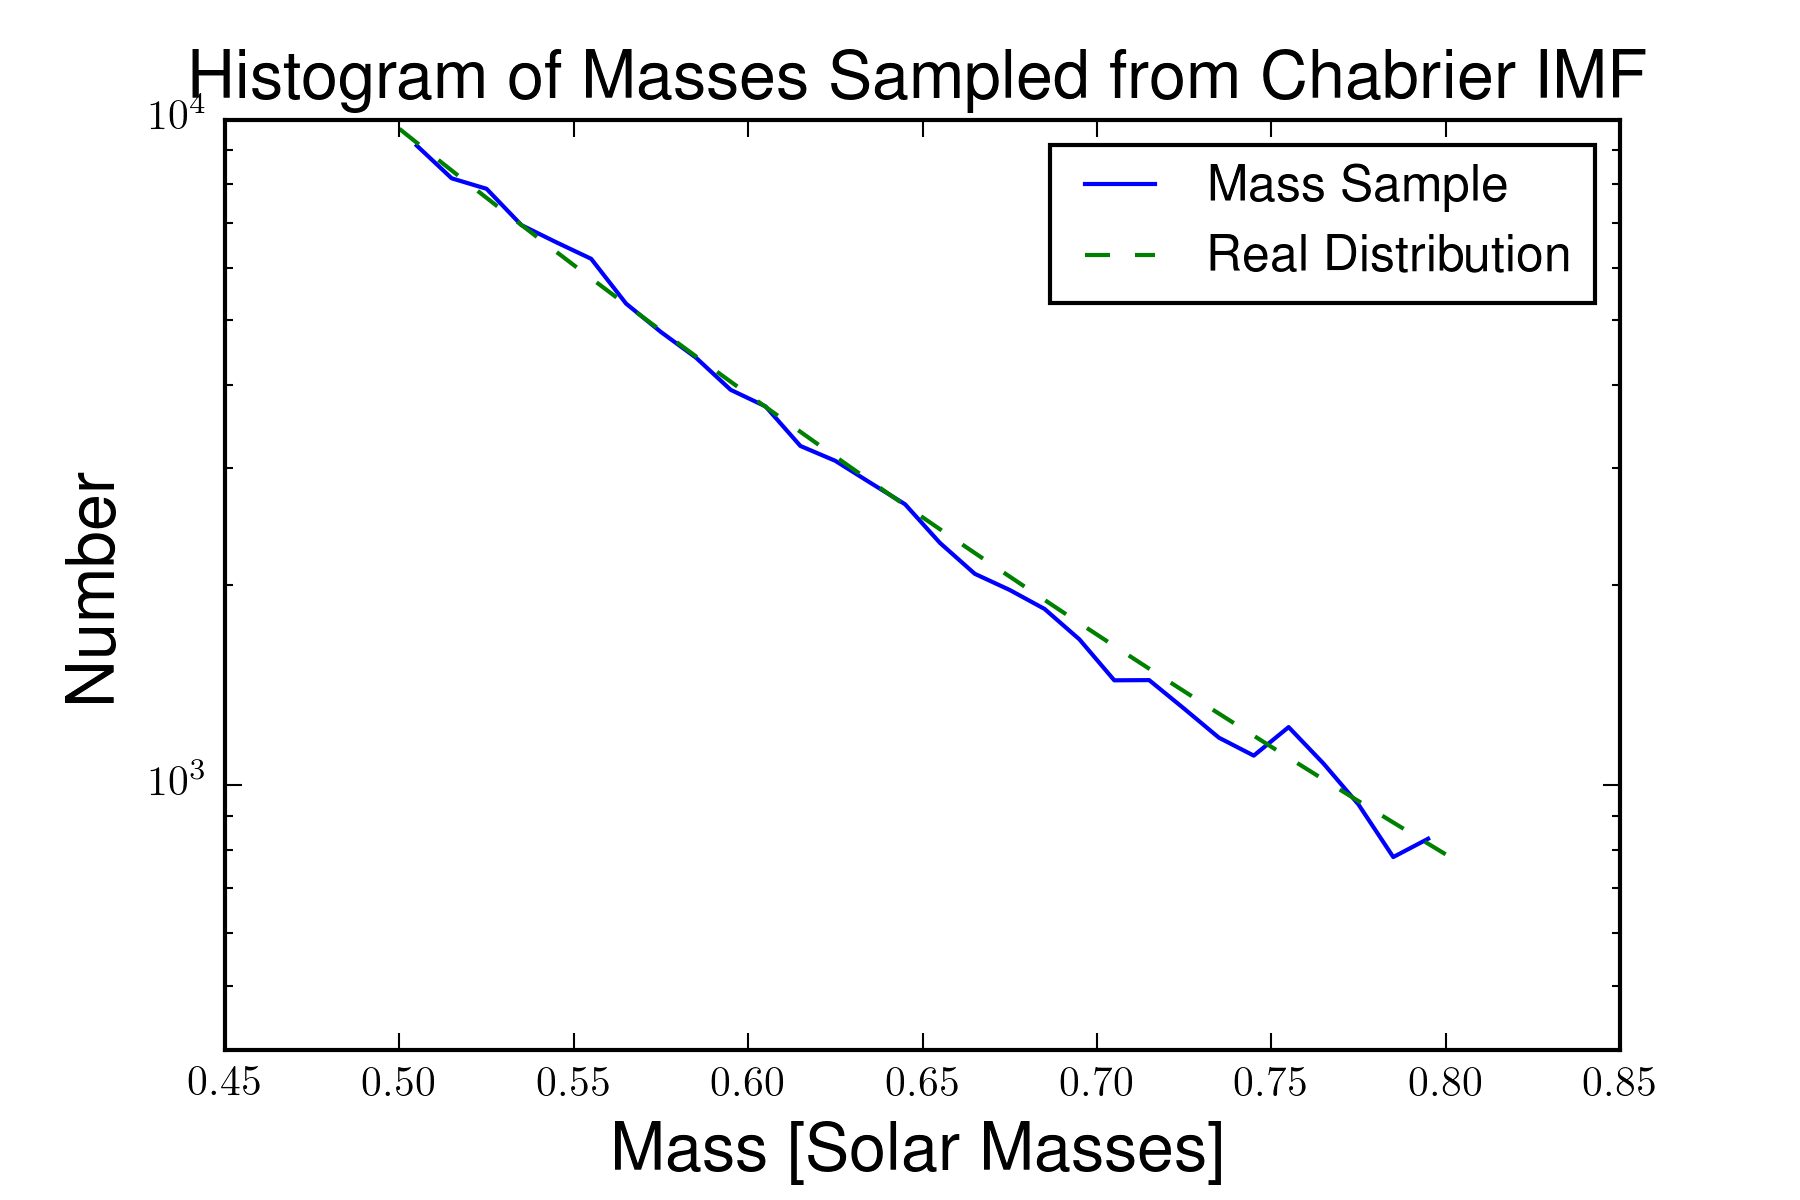
\includegraphics[scale = 0.6]{histogram_of_masses_chabrier_prob4.png}
\end{figure}

\subsection*{(b)}
\textit{Now, assuming a single-slope power-law IMF model (as done with the literature), infer the value of the spectral index $\alpha$. How does this compare with the canonical Kroupa IMF found in the Milky Way?}

For this problem I used emcee to fit the slope of a single-slope power-law to the data. The contour plot of the result is below.

\begin{figure}[H]
\centering
\caption{Slope Value for Fitting Power Law to Chabrier IMF}
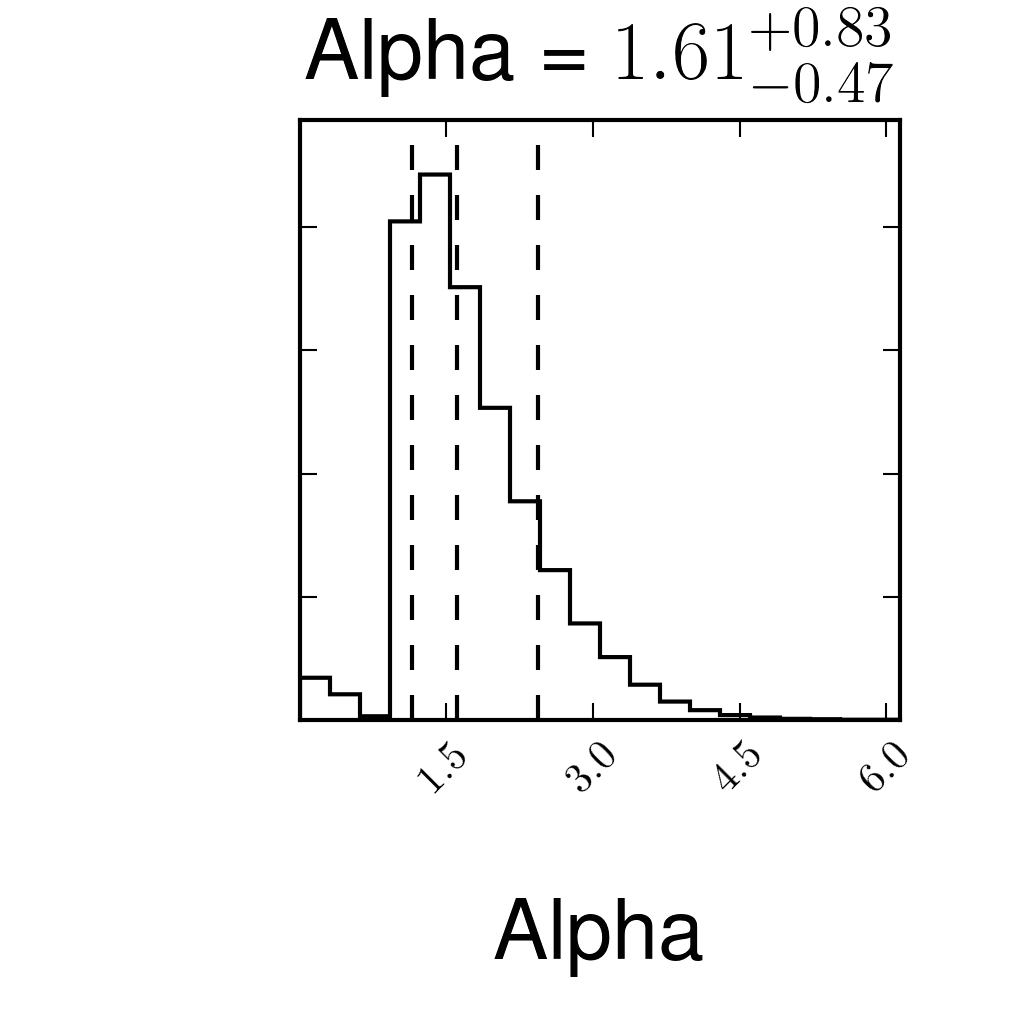
\includegraphics[scale = 0.6]{corner_plot_emcee_prob4.png}
\end{figure}
Kroupa had an $\alpha$ slope of 2.3 for mass greater than 0.5 solar masses. The value I found it around $\alpha$ = 1.61. This is lower than the Kroupa IMF and likely is a result of wrongly trying to fit a power law to a distribution that is actually log normal.

\section*{Problem 5}

\subsection*{(1)}
\textit{Generate the spectrum for a 10 Myr simple stellar population (assume no dust, fixed metallicity, etc- the only variable of interest is age). Plot how the spectrum from 1500 - 10000 $\AA$ changes for three different high-mass IMF (>1$M_{\odot}$) values: $\alpha$ = 0.8, 1.3, 1.8, holding the lower portions of the IMF fixed.}\\

\begin{figure}[H]
\centering
\caption{Spectrum for Varying $\alpha$ in the High-Mass IMF}
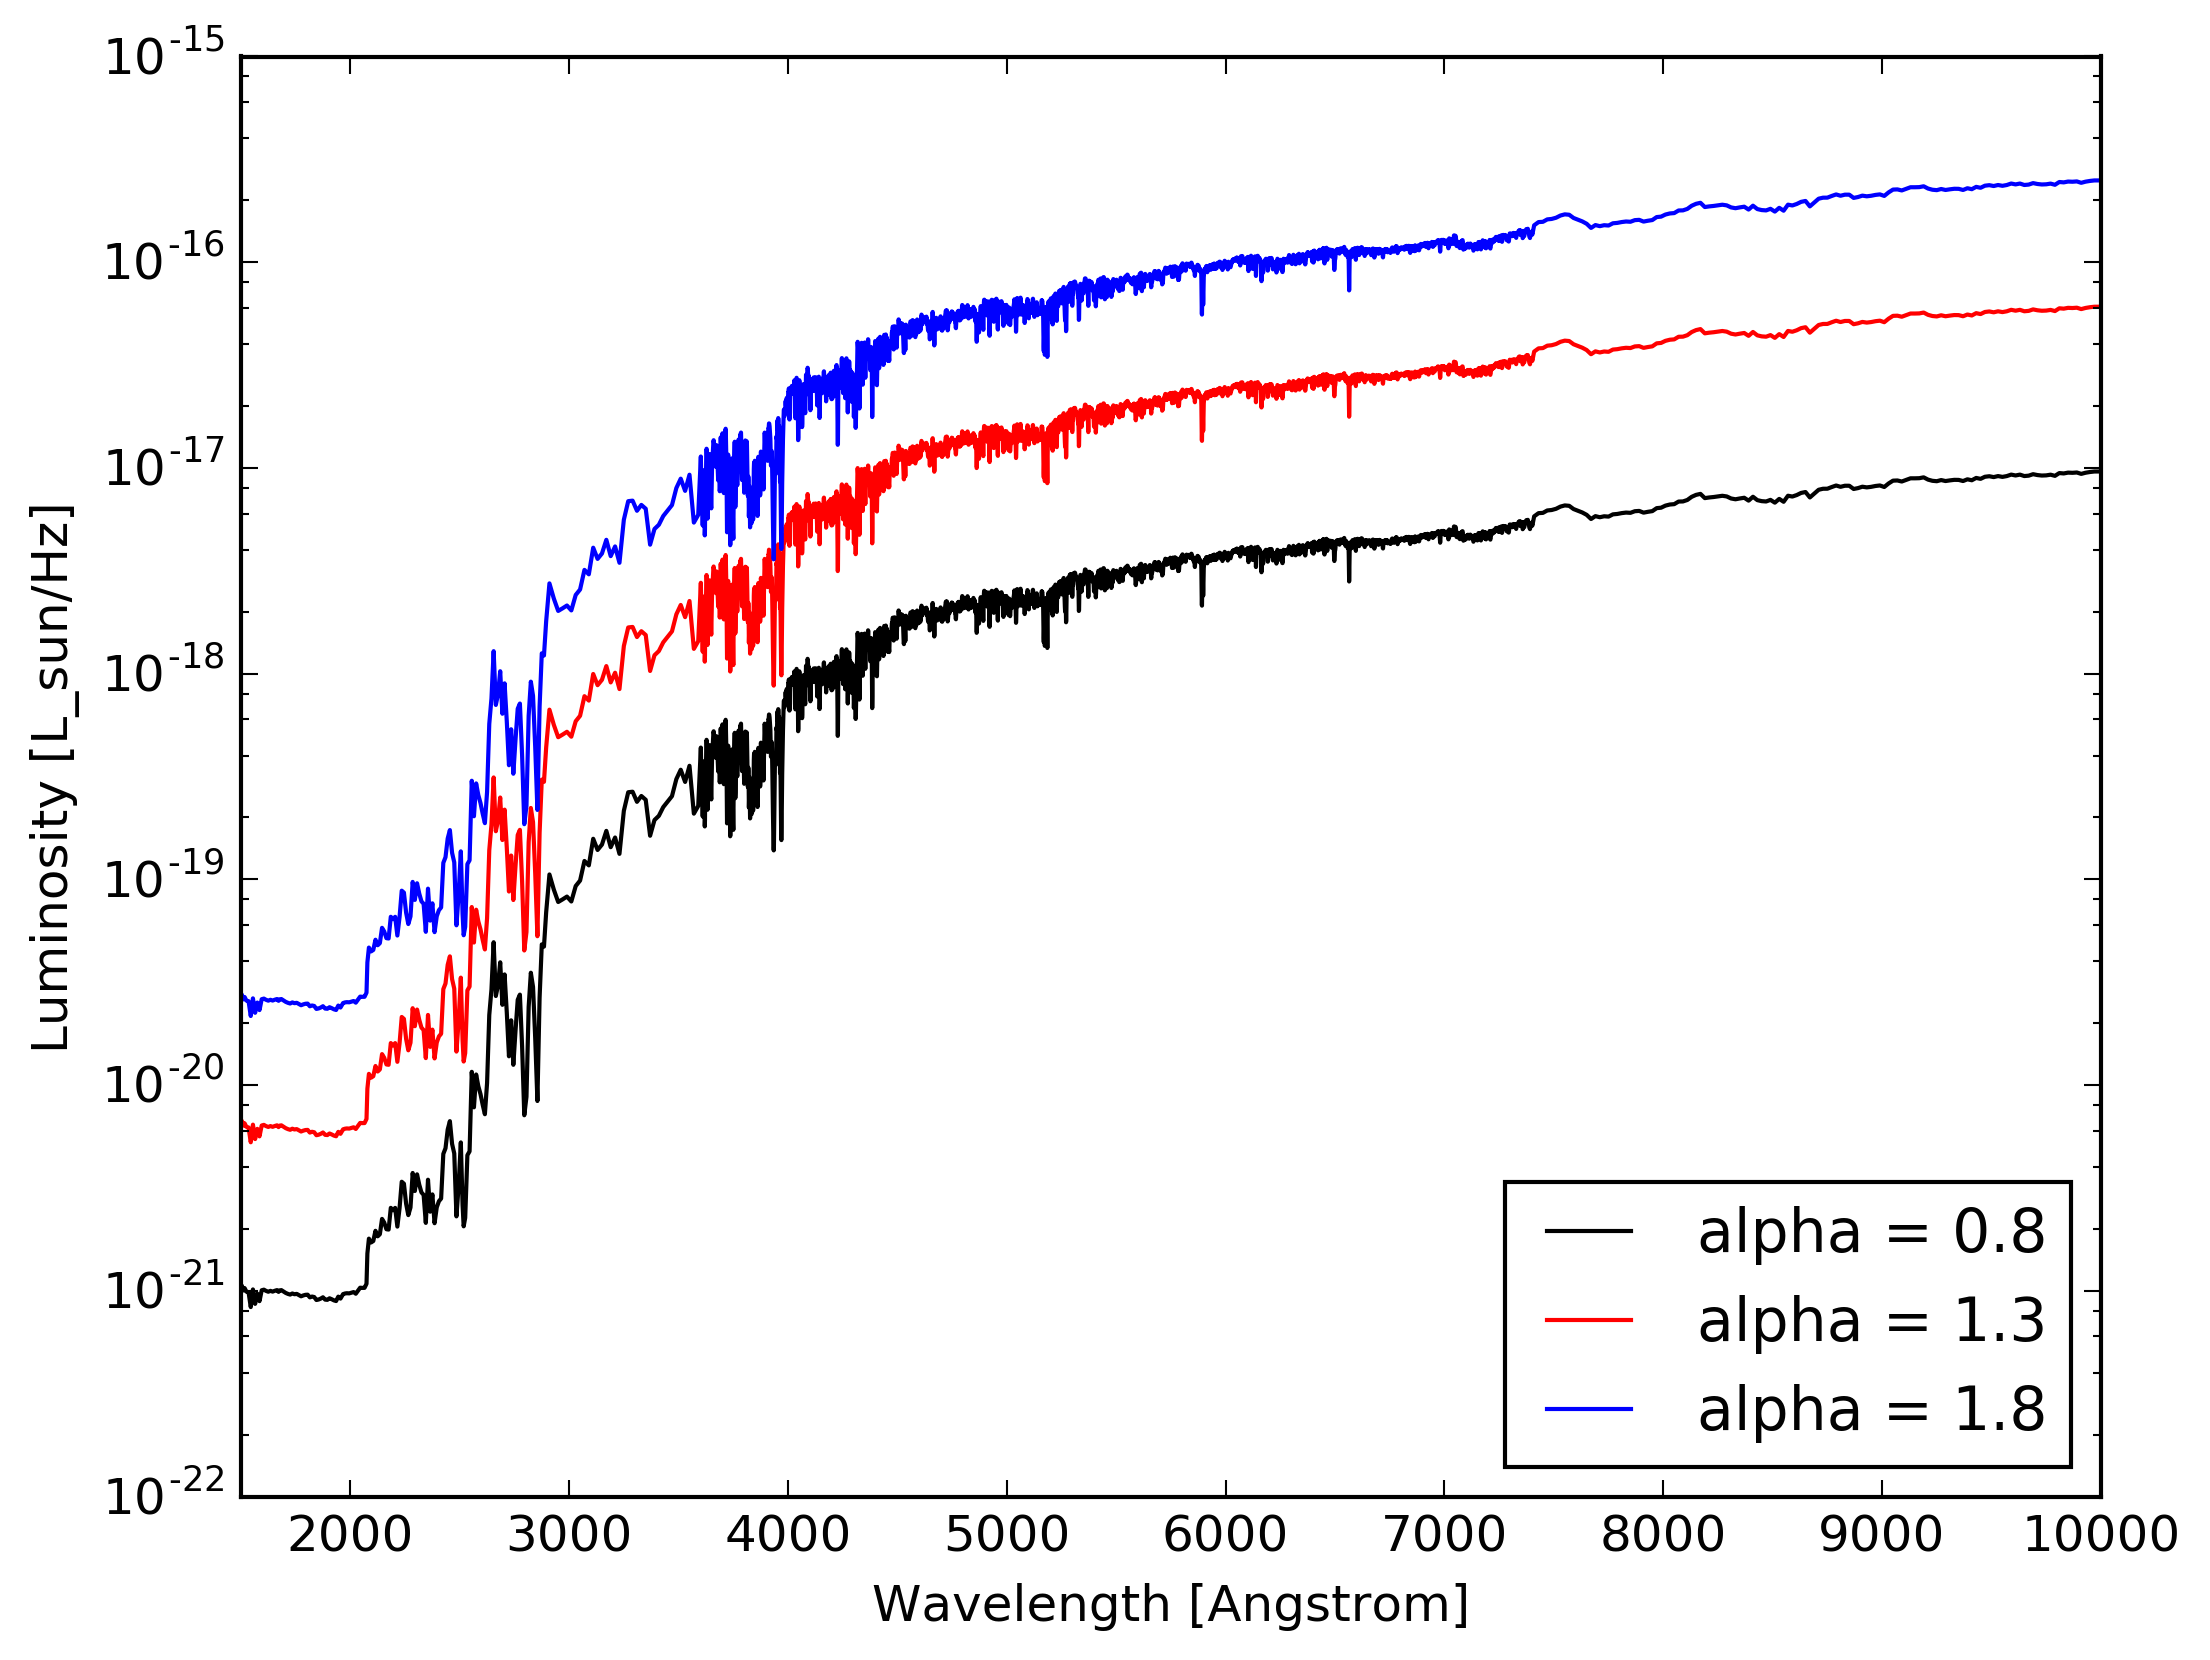
\includegraphics[scale = 0.6]{spectra_varying_alpha_problem_5.png}
\end{figure}


\subsection*{(2)}
\textit{Generate the spectrum of a 10 Gyr simple stellar population. Plot how the spectrum from 5000-20000 $\AA$ changes for three different IMF forms: Salpeter IMF, a Kroupa IMF and the van Dokkum IMF.}\\

\begin{figure}[H]
\centering
\caption{Spectrum for Varying IMF in Simple Stellar Population}
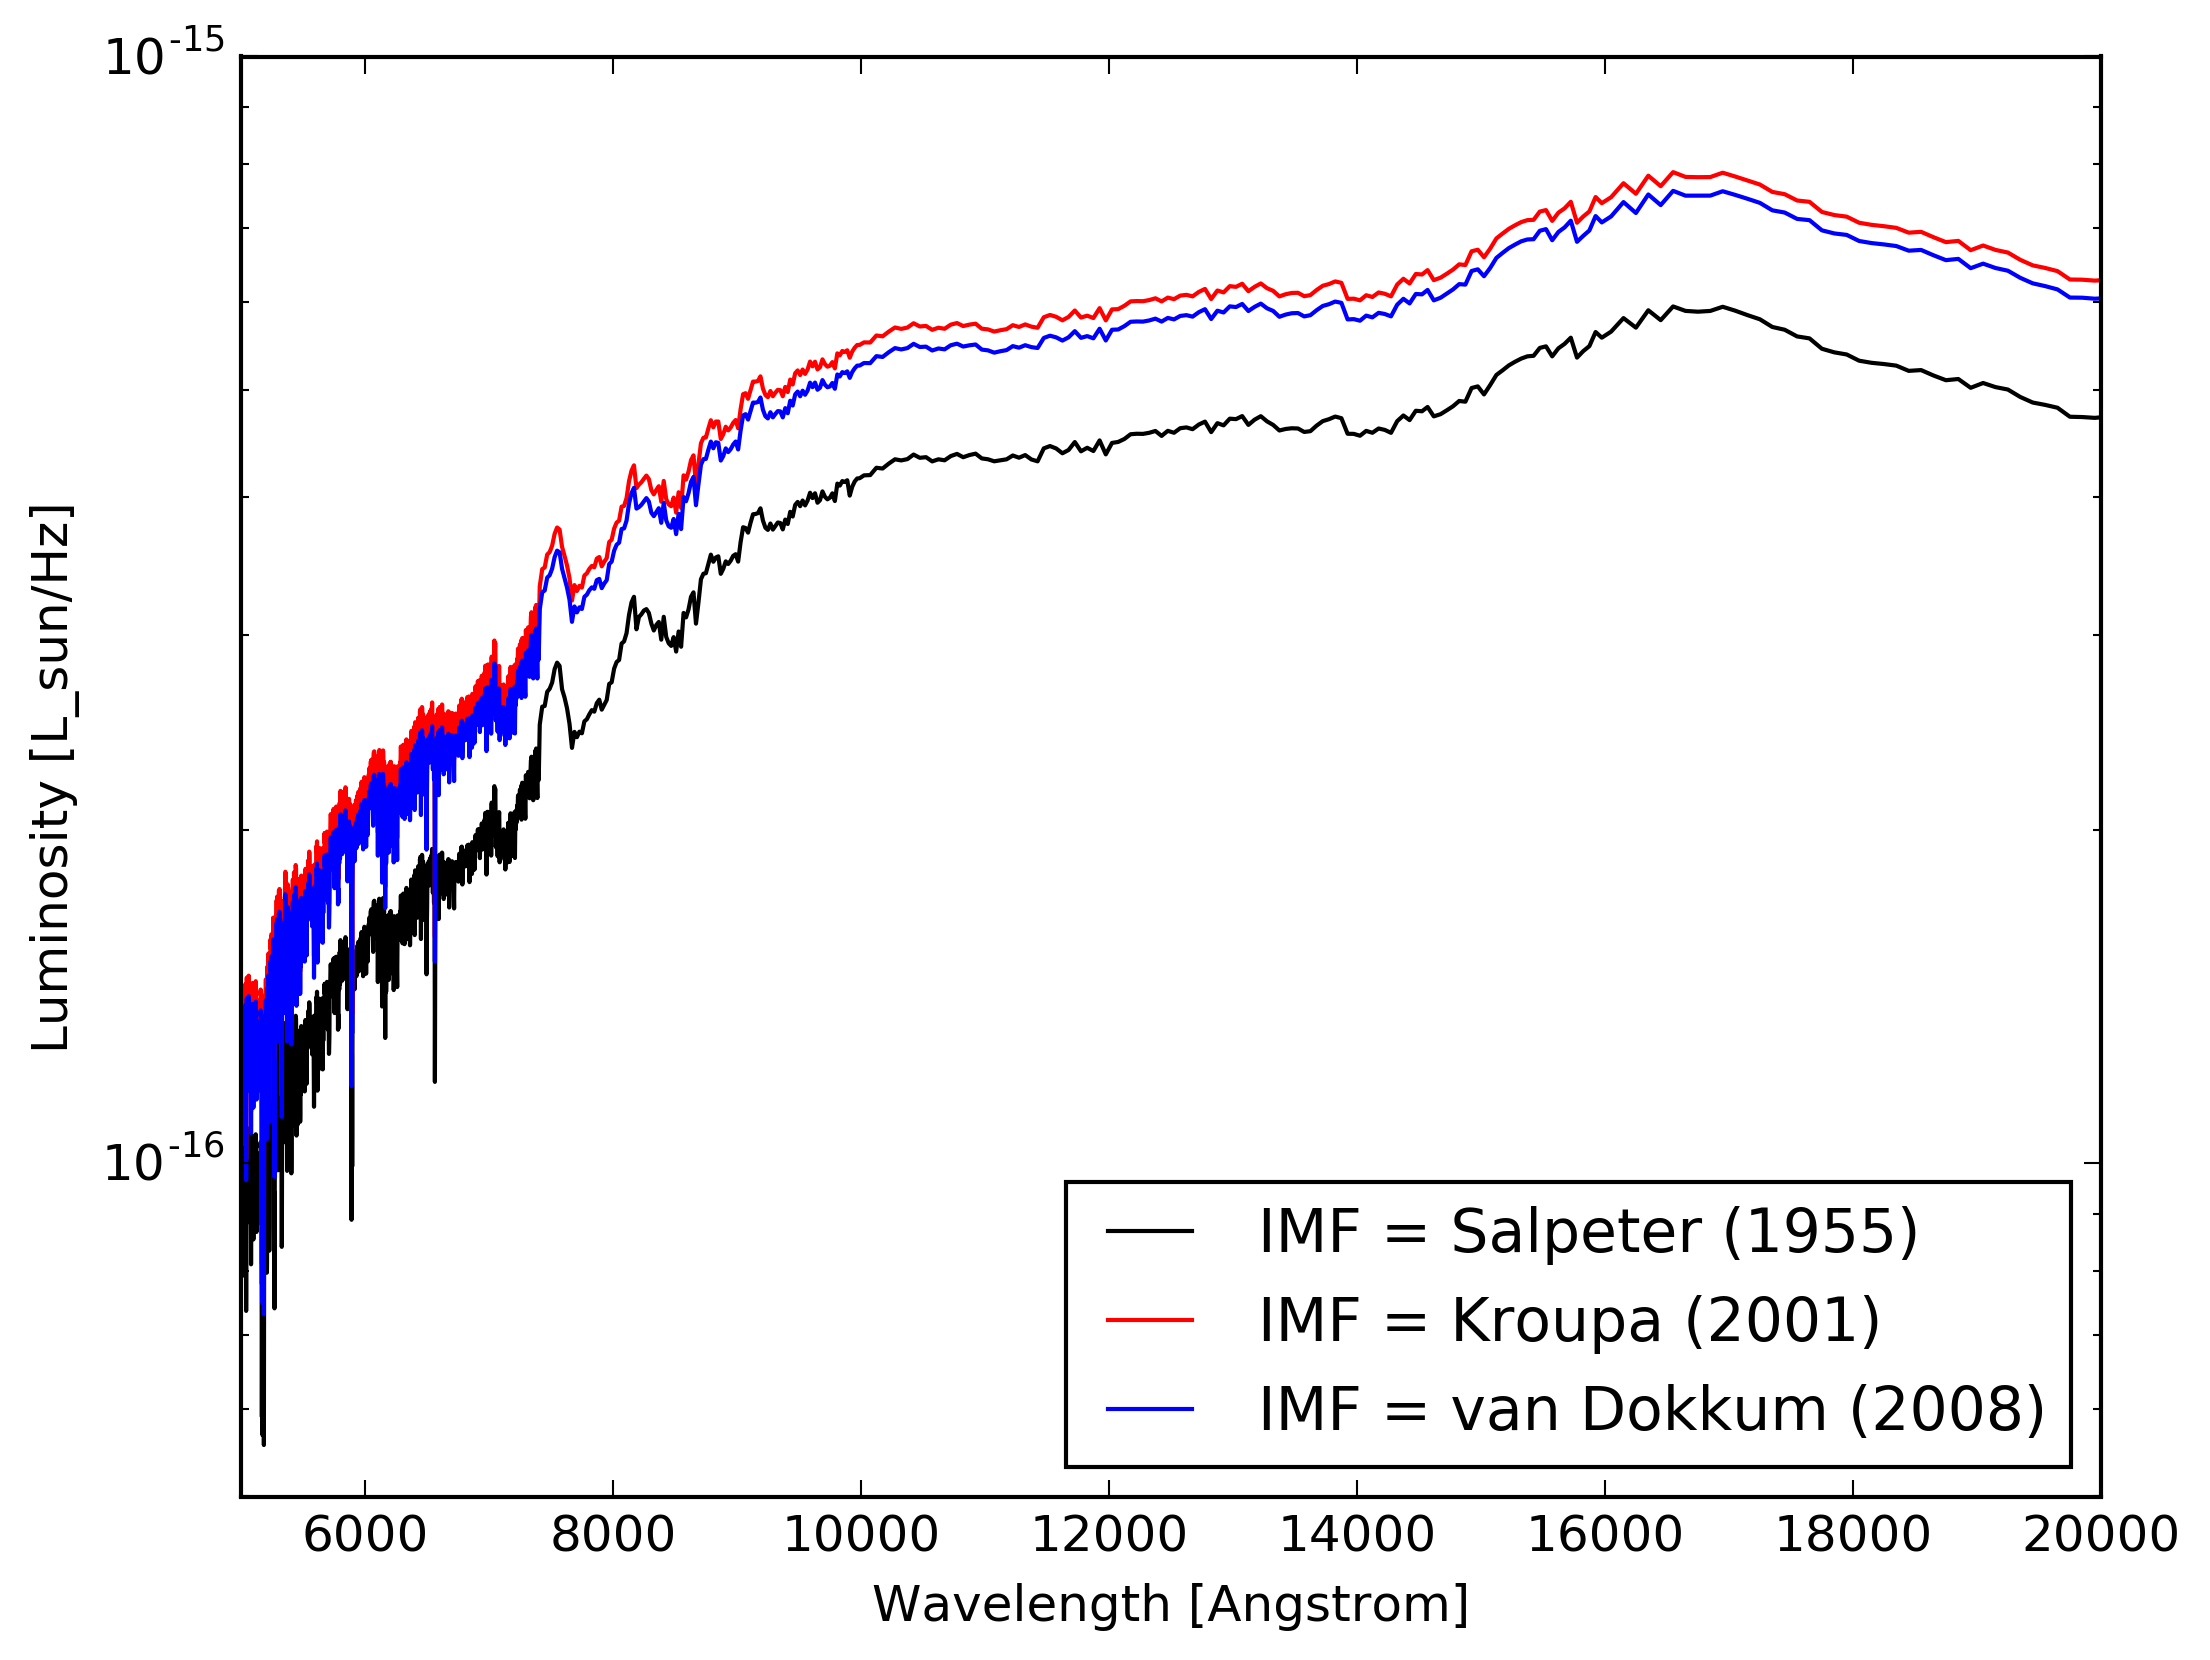
\includegraphics[scale = 0.6]{spectra_varying_imf_problem_5.png}
\end{figure}




\end{document}